%!TEX root = ../dissertation.tex
\begin{savequote}[75mm]
Half the variations which are calculated in a tournament game turn out to be completely superfluous. Unfortunately, no one knows in advance which half.
\qauthor{Jan Timman}
\end{savequote}

\Chapter[Rational use of cognitive resources in human planning\footnote{
  This chapter is based on the following paper:\newline\bibentry{callaway2022rational}.%
}]{Planning}\label{sec:planning}


\newthought{One of the hallmarks} of human intelligence is our ability to act adaptively in novel and complex environments. It is widely agreed that this ability depends critically on our ability to plan, that is, to use a model of the world to simulate, evaluate, and select among different possible courses of action. Research in psychology \citep{huys2015interplay,huys2012bonsai,vanopheusden2017computational,macgregor2001information,keramati2016adaptive,krusche2018adaptive,snider2015prospective}, economics \citep{vonneumann1944theory,stahl1994experimental,camerer2004cognitive} and computer science \citep{newell1956logic} has formalized planning as search over a ``decision tree'', where every decision one might have to make is represented as a branching point (see \figref{fig:planning-model}{}). In principle, one can identify the best plan by considering every possible decision point. However, traversing the full decision tree is infeasible because the size of the tree grows exponentially with the number of steps that one looks ahead.

The question of how people are able to effectively plan in the face of such formidable computational obstacles is of great interest for both researchers who wish to understand human intelligence and those who wish to recreate it \citep{griffiths2019doing}. In fact, one of the earliest attempts to replicate human-like intelligence in a computer, conducted by Newell and Simon, focused on problems that require thinking multiple steps ahead \citep{newell1956logic,newell1959report,newell1972human}. Even at this early stage, it was immediately recognized that the success of human planners (and any hope for success of artificial planners) depended critically on the use of heuristics to circumvent the exponential growth of search trees. Recent work on human planning has largely followed a similar vein, proposing and testing different possible heuristics people could be using to reduce the cost of planning. For example, people might limit the depth of their search \citep{macgregor2001information,keramati2016adaptive,krusche2018adaptive,snider2015prospective}, ``prune'' away initially unpromising courses of action \citep{huys2012bonsai,huys2015interplay}, or avoid planning altogether by relying on habit or ``memoization'' \citep{huys2015interplay,kool2017costbenefit}. Each of these models provides insight into how people circumvent the computational intractability of planning. 

Despite these successes, the approach of postulating and testing specific heuristics faces several challenges. First, it is limited by the creativity of the researchers who must generate hypotheses about different possible heuristics people could be using. Second, it does not provide a straightforward way to predict which heuristics will be employed in new situations, or how each individual heuristic should be parameterized (e.g., How deep will someone plan in this environment? How large of a punishment will lead to a branch being pruned?) Finally, although these models are intuitively motivated as making planning more efficient, they do not provide a formal answer to the question of why people use these heuristics \citep{norris2021more}.

These challenges---hypothesis generation, generalizable prediction, and functional explanation---are not unique to planning; indeed, they arise in nearly all areas of cognition. In many domains, progress in addressing these challenges has been made by analyzing optimal solutions to the problem a cognitive system is meant to solve \citep{marr1982vision,anderson1990adaptive}. This approach has generated insight into a wide range of problems, including decision-making \citep{savage1954foundations}, generalization \citep{tenenbaum2001generalization}, categorization \citep{anderson1991adaptive,ashby1995categorization}, perception \citep{knill1996perception}, and information-seeking \citep{oaksford1994rational,gureckis2012selfdirected}. More recently, the notion of optimality has been extended to account not only for the demands imposed by the external environment but also the demands imposed by our own cognitive limitations \citep{howes2009rational,lewis2014computational,gershman2015computational,griffiths2015rational,lieder2020resourcerational}. This approach dates back to Simon \citep{simon1955behavioral} and has been especially useful in the domain of decision-making, where it has been used to explain both how long people deliberate \citep{bogacz2006physics,drugowitsch2012cost,tajima2016optimal,tajima2019optimal,fudenberg2018speed} and also what people think about \citep{callaway2021fixation,jang2021optimal} while making ``simple'' (i.e., non-sequential) choices. However, to the best of our knowledge, there has been no such analysis in the domain of planning, despite the especially critical role that computational limitations play in this case (but c.f. \citealp{sezener2019optimizing,mattar2018prioritized} for closely related efforts, which we discuss further below).

In this work, we propose an optimal model of planning under computational constraints. Drawing on the field of rational metareasoning in artificial intelligence \citep{matheson1968economic,horvitz1987reasoning,russell1991principles}, we formalize planning as a sequential decision problem in which an agent executes a sequence of cognitive operations to construct a decision tree. Formalizing planning in this way allows us to identify the optimal planning strategy for a given environment as the one that maximizes the expected utility of executing the resulting plan minus the cost of each cognitive operation used to make that plan. This also provides a flexible framework for specifying heuristic planning strategies in a highly precise and composable way. Every model we consider specifies an explicit distribution over the sequence of planning operations that will be executed in any given environment.

To rigorously test the fine-grained predictions of the optimal and heuristic models, we develop a novel process-tracing paradigm that externalizes the cognitive operations underlying planning as mouse clicks, extending the widely used Mouselab paradigm \citep{payne1976task} to sequential decision-making problems. In a series of four experiments, we find that our participants use planning strategies that are largely consistent with optimal planning strategies, using previously proposed heuristics when they are adaptive, but adjusting their strategies when the structure of the environment changes. However, we also find systematic deviations from optimal planning, in particular a bias towards considering states in the order in which they would be traversed (forward search). Based on these results, we conclude that human planners use highly adaptive planning strategies, but that these strategies are also shaped by additional constraints that may reflect the specific cognitive mechanisms underlying human planning.

\begin{figure}[ht]
    \centering
    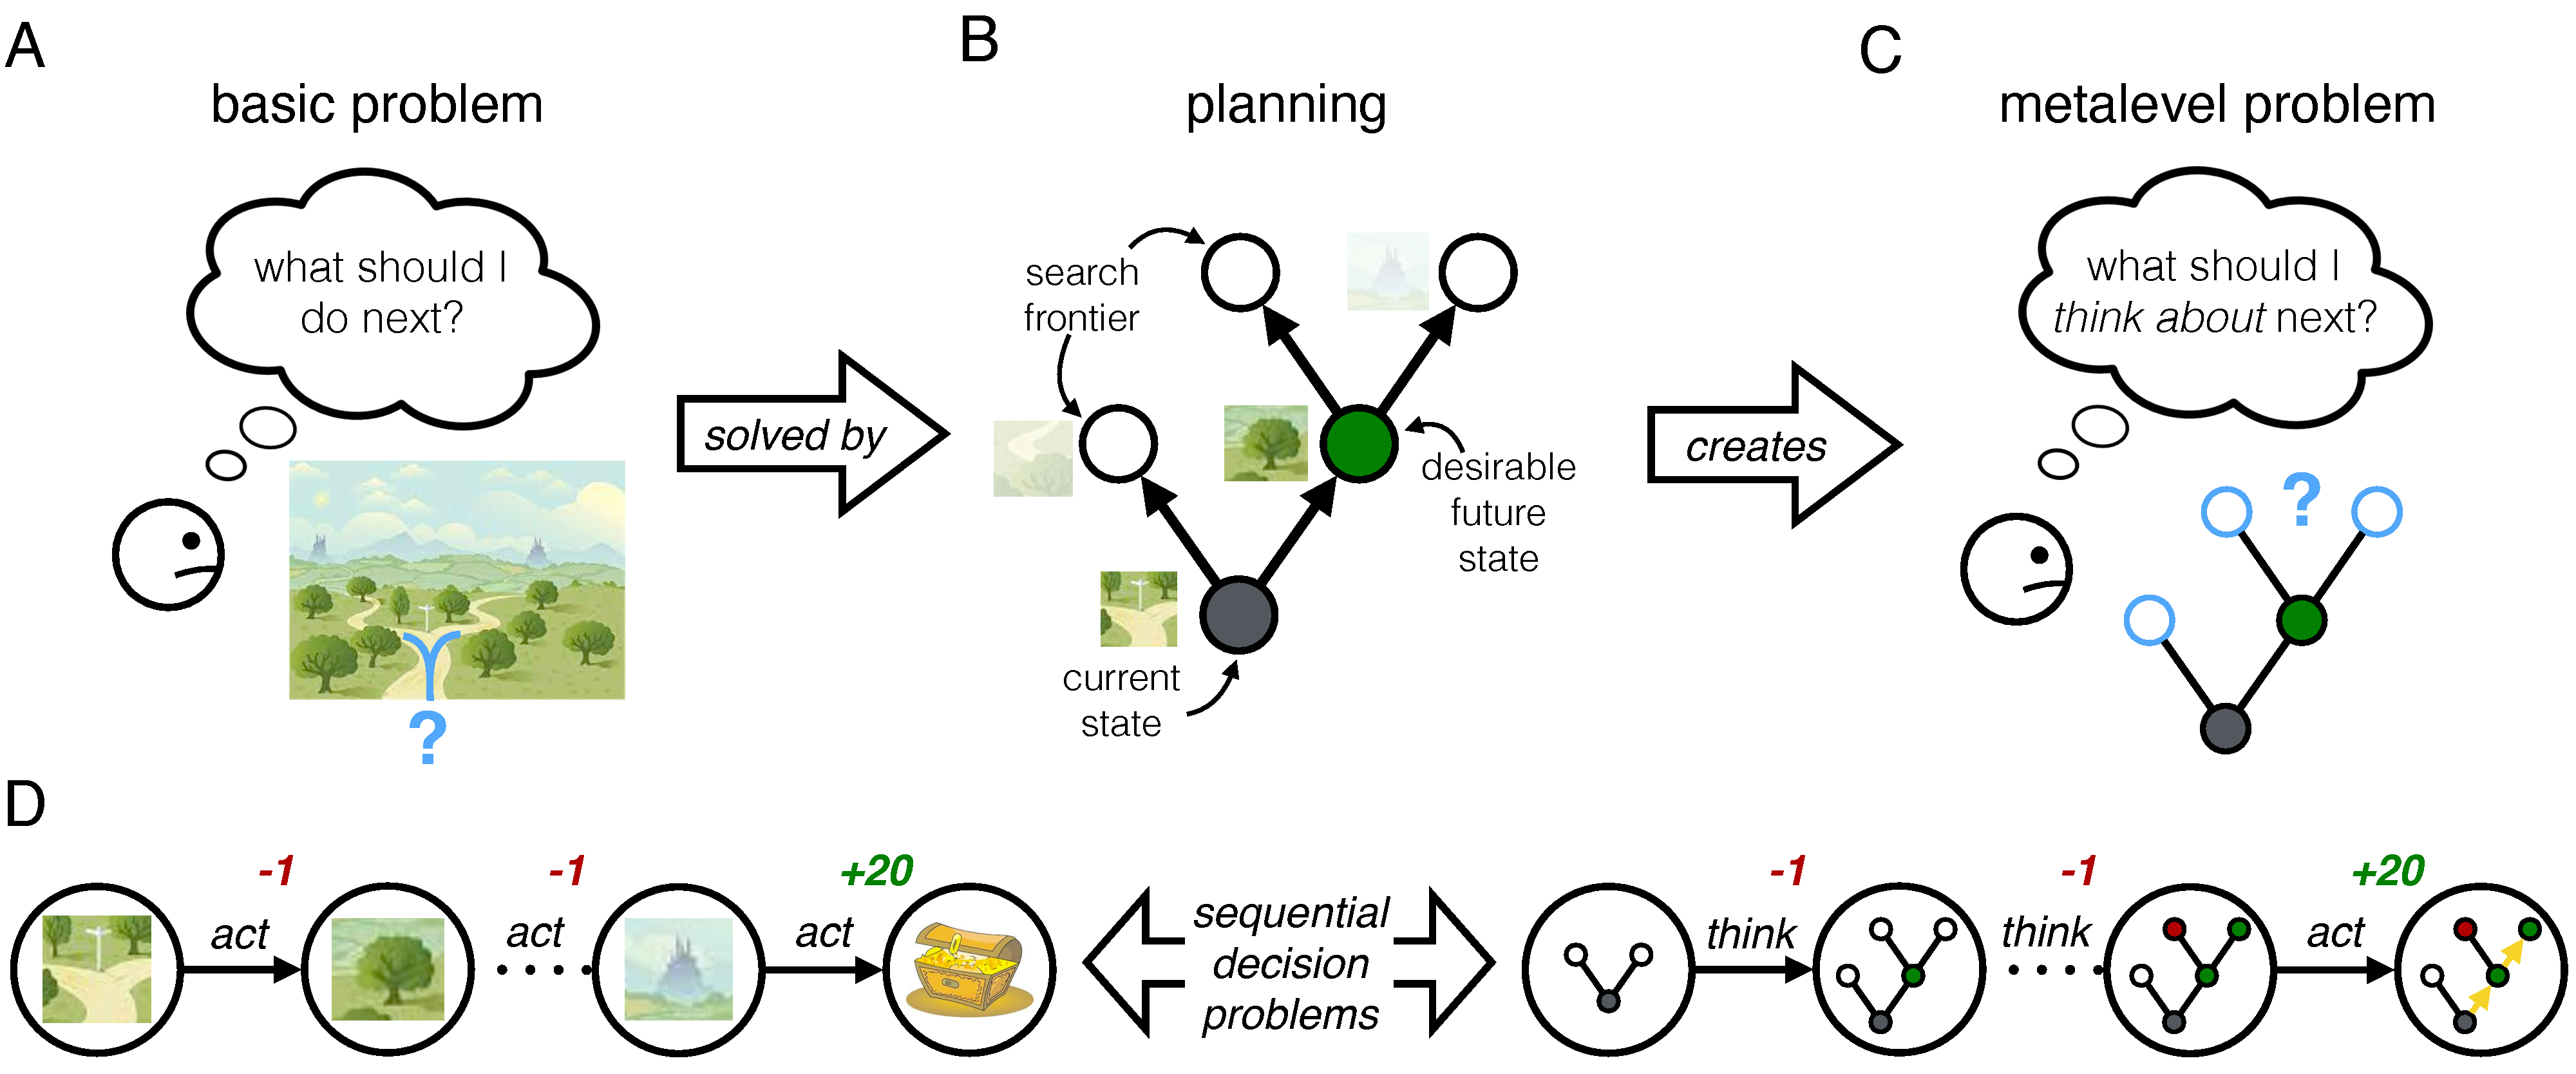
\includegraphics[width=\textwidth]{figs/planning/fig1.pdf}
    \caption{\captiontitle{Formalizing planning under computational constraints.}
      \subcap{A} The basic problem facing an intelligent agent is to take actions that maximize long-run reward. If the agent can predict the consequences of their actions, they can solve this problem by planning.
      \subcap{B} In one version of planning, the agent constructs a decision tree where nodes (circles) represent possible future states and edges (arrows) represent possible actions the agent could take. The agent constructs the tree by iteratively considering possible future states, estimating the reward to be gained there, and expanding the search frontier to include states that could be visited next. Eventually, this procedure will reveal the sequence of actions that maximize reward. But for an agent with limited cognitive resources, exploring the entire tree is usually infeasible. 
      This creates the metalevel problem:
      \subcap{C} Which states should the agent consider---or ignore---in order to achieve the best tradeoff between the costs and benefits of planning?
      \subcap{D} The key observation underlying our model is that the basic problem and the metalevel problem are both sequential decision problems. 
      That is, they require the agent to make a sequence of choices, in which the outcome of each choice depends on which choices were made previously. 
    }
    \label{fig:planning-model}
\end{figure}

\section{Model}\label{sec:planning-model}

Following previous work \citep{huys2012bonsai,huys2015interplay,vanopheusden2017computational,sezener2019optimizing}, we model planning as search over a decision tree. That is, we assume that the agent represents possible courses of actions as a tree-structured directed graph, in which nodes correspond to hypothetical future states and edges correspond to actions that bring the agent from one state to another (\figref{fig:planning-model}{b}). By constructing such a tree and passing information about future rewards back to the root node (representing the current state), the agent can determine a sequence of actions that maximizes total reward. However, constructing the entire tree is prohibitive in large problems. How should a resource-constrained agent plan in such a setting?

One intuitive way to conceptualize the problem of resource-constrained planning is in terms of a cost-benefit tradeoff \citep{daw2005uncertaintybased,keramati2011speed,shenhav2013expected,kool2017costbenefit,kool2018mental} in which an agent must find an optimal balance between the mental effort or time spent planning and the quality of the resulting decision. This type of model predicts, for example, that people will reduce the depth of planning under time pressure \citep{keramati2016adaptive}. However, this one-dimensional simplification cannot capture the full range of different planning strategies people might employ. In particular, a planning strategy specifies not only the amount but also the direction of planning, that is, which courses of action are explored deeply and which are hardly considered at all \citep{sezener2019optimizing}. To further complicate matters, it is not sufficient (or perhaps even possible) to determine in advance the amount and direction of planning. An adaptive planning strategy will dynamically adjust both based on the partial results of previous planning; for example, one can only prune away a branch of a decision tree after discovering a large punishment early on that branch \citep{huys2012bonsai}.

To summarize, the problem of planning involves balancing between costs and rewards attained at different time points, by determining in which direction to plan (or to stop planning) based on the outcome of previous planning. That is, in addition to being a method for solving sequential decision problems, planning is itself a sequential decision problem (\figref{fig:planning-model}{}). This is exactly the insight captured by the metalevel MDP framework. Below, we define a metalevel MDP model of decision-tree search.

\subsection{Metalevel Markov decision process}

To characterize optimal resource-constrained planning, we cast decision-tree search as a metalevel MDP in which the mental states correspond to partially constructed decision trees and the computations correspond to expanding a node in the tree. We detail the five components of the metalevel MDP below.

\paragraph{A note on terminology}

So far, we have used the term ``state'' to refer to states in the \emph{object-level} MDP, that is, the one that defines the planning problem itself. For example, in Figure~\ref{fig:planning-model}, the object-level states are physical locations. Critically, the object-level states are different from the world state (defined below). When it is clear from context, we will continue to use ``state'' to refer to the object-level states. We will use the term ``object-level reward'' to refer to the rewards associated with the object-level MDP.

\paragraph{World states}

The world state defines the object-level reward that the agent would receive in each object-level state. Following Chapter~\ref{sec:attention}, we denote the reward associated with object-level state $i$ as $u^{(i)}$.\footnote{%
  This notion of world state may be counter-intuitive at first, as it is really defining the object-level reward function. Note, however, that this is the natural generalization of the world state in Chapter~\ref{sec:attention} (which specified the utility of each item in the choice set) to a sequential object-level problem.
} We assume that the object-level environment has $n$ states; the world state is thus represented as a vector of length $n$. 

\paragraph{Mental state}

The mental state $m$ corresponds to a partially constructed decision tree. We make the simplifying assumptions that the external environment is itself tree-structured and known to the agent.\footnote{%
  This is really quite a simplifying assumption, but also a very challenging one to not make. \citet[Section 5.2]{hay2016principles} presents a sophisticated recursive method for representing search trees of arbitrary size. Such a method could be used to create cognitive models that do not make this assumption.
} Thus, the largest possible decision tree has the same graphical structure as the environment itself. The mental state can thus be represented as a vector of length $n$ where each position corresponds to a node in the decision tree. The values $m^{(i)}$ specify either the reward that can be attained at the object-level state $i$, or a special value $\oslash$, which indicates that the corresponding node has not been expanded yet. In the initial mental state, only the root node (the initial object-level state) has been expanded, always having value $0$; all other nodes have value $\oslash$.

\paragraph{Computations}

A computation $c$ corresponds to expanding a node of the decision tree. This operation determines the cost or reward for visiting an object-level state and integrates that value into the total value of the path leading to that state. There is thus one computation $c^{(i)}$ to expand each node $i$. In standard decision-tree search, one can only expand nodes that are connected to nodes one has already expanded, the \emph{search frontier}. That is, one can only consider actions in states that are already explicitly represented in the tree. Formally, we define
\begin{equation}
\frontier(m) = \{c^{(i)} \mid m^{(i)} = \oslash \wedge m^{(\mathrm{parent}(i))} \neq \oslash \}
\end{equation}
and limit the set of allowable computations in mental state $m$ to $\frontier(m)$. Here, $\mathrm{parent}(i)$ is the parent node of the expanded node, corresponding to the state from which the newly considered state can be reached. Note that, for ease of notation, we have defined $\frontier(m)$ as the set of allowable computations rather than the nodes themselves.

% As in all metalevel MDPs, there is an additional operation, $\bot$, that terminates the computation process.  Upon terminating planning, the agent executes an action sequence that has maximal expected value according to the decision tree it has built up until that point (specified further below).

\paragraph{Transition function}

The metalevel transition function specifies the effect of node expansion on the decision tree. If $c^{(i)}$ is executed in $m_t$, the resulting mental state is identical to $m_t$ except that the entry for node $i$ is set to the true object-level at node $i$:
\begin{equation}
  m_{t+1}^{(i)} = u^{(i)}.
\end{equation}
The marginal transition function is identical, except that $u^{(i)}$ is sampled from a node-specific distribution $U^{(i)}$ capturing the agent's prior knowledge about the distribution of rewards in the environment. This distribution is a key aspect of the environment that we will manipulate in Experiments~2 and~3.

\paragraph{Reward function}

The metalevel reward function captures both the cost of node expansion and the quality of the plan that is ultimately executed. We assume that node expansion has a fixed cost, $R(m, c) = \gamma$. To capture plan quality, the reward for the termination operation is the value of the external rewards one will attain while executing the chosen plan (a sequence of object-level states). We assume that the plan is selected optimally given the current decision tree. For this model, we directly specify the marginal termination reward, which is the maximum expected value of any complete plan\footnote{%
  Note that a complete plan generally cannot be computed given a partial decision tree. Our assumption of maximizing over the expected value of complete plans corresponds to the assumption that, when the agent reaches a frontier node, they fall back on a default policy that is sensitive only to the expected reward at different states. In Experiments~1-3, this expected reward at all states is zero, and so it can be ignored. In Experiment 4, the expected reward is strictly negative but constant across states, so it corresponds to following the shortest path to the terminal state. This assumption is consistent with the broader assumption that the agent has direct knowledge of the transition structure and reward distributions. Addressing the more realistic case in which these are not known is an important direction for future research.
} (i.e., one ending in a terminal state) given the current decision tree:
\begin{equation}
R(m, \bot) = \max_{p \in \P} V(m, p),
\end{equation}
where $\P$ is the set of possible complete plans (all possible trajectories from the initial state to a terminal state) and $V$ specifies the expected value of a plan:
\begin{equation}
  V(m, p) = \sum_{i \in p} 
\begin{cases}
\E[U^{(i)}] &\mathrm{if\ } m^{(i)} = \oslash \\
m^{(i)} &\mathrm{otherwise}.
\end{cases}
\end{equation}

% \footnote{Note that the identity of the best plan is updated by each node expansion operation, and thus the selection of the best plan involves little additional computation.}

\subsection{Optimal and heuristic policies}
We have now specified all four components of a metalevel MDP for decision-tree planning. However, there are countless possible planning algorithms consistent with this general class. To create a complete model, we must specify one additional component: the strategy one uses to select which nodes to expand, and when to stop expanding nodes. Formally, this corresponds to a policy for the metalevel MDP, a distribution over computations in each possible mental state.

One policy of particular interest is the optimal policy, that is, the one that maximizes the expected total metalevel reward. On a given trial, the total metalevel reward is the external reward attained by executing the chosen plan minus the cost of the node expansions used to construct the plan. The optimal policy thus balances the costs and benefits of search, expanding the nodes that are most likely to improve one's ultimate decision, and only doing so when the expected improvement in decision quality outweighs the cost of expansion.  Importantly, the optimal balance depends on the cost of node expansion; the optimal model's behavior is thus governed by one key free parameter (not including parameters of the noise/lapse model used to fit human data; see Section~\ref{sec:planning-modelspec}).

Early work in rational metareasoning proposed that optimal metalevel policies can be approximated by a myopic one-step lookahead (\citealp{russell1991principles}; Section~\ref{sec:myopic}). The myopic policy chooses the planning operation that would be most helpful if the agent had to select a plan immediately afterward. Like the optimal model, this model has one key free parameter, the cost of node expansion.

We additionally consider ``heuristic'' policies based on three classical planning algorithms \citep{russell2002artificial}. Breadth-first search first considers all immediate successors of the current state, then the successors of those states, and so on. That is, it prioritizes nodes that are close to the initial state. In contrast, depth-first search constructs a full plan to a terminal state before considering any alternative; it prioritizes nodes that are far from the current state. Finally, best-first search prioritizes nodes on promising paths, that is, nodes that lie on the frontier of plans with high expected value.

These classical algorithms specify the order in which nodes are expanded, but are agnostic about how people might decide when to stop planning. Previous research has proposed a number of heuristics people might use to reduce the amount of planning they must do to reach a decision. We consider four such heuristics. The ``satisficing'' heuristic terminates planning as soon as it finds a path whose expected value exceeds some predefined threshold \citep{simon1955behavioral}. The ``best vs. next'' heuristic terminates planning when one path's expected value is sufficiently greater than any other path's \citep{solway2015evidence}. As discussed below, these two terms respectively correspond to absolute and relative stopping rules in evidence accumulation models. The pruning heuristic stops considering paths once their value falls below a predefined threshold \citep{huys2012bonsai}. The ``depth limit'' heuristic only considers states that can be reached in some predefined number of steps \citep{macgregor2001information,keramati2016adaptive,krusche2018adaptive,snider2015prospective}. For brevity, we will refer to these heuristic mechanisms for limiting the amount of planning as simply ``heuristic mechanisms''. We assume that people could use any combination of these four mechanisms, resulting in $3 \times 2^4 = 48$ heuristic planning models (three search orders and sixteen combinations of heuristic mechanisms for each). The heuristic models have between $3$ and $9$ parameters depending on which mechanisms are included (see Section~\ref{sec:planning-modelspec}).

\begin{figure}[t!]
    \centering
    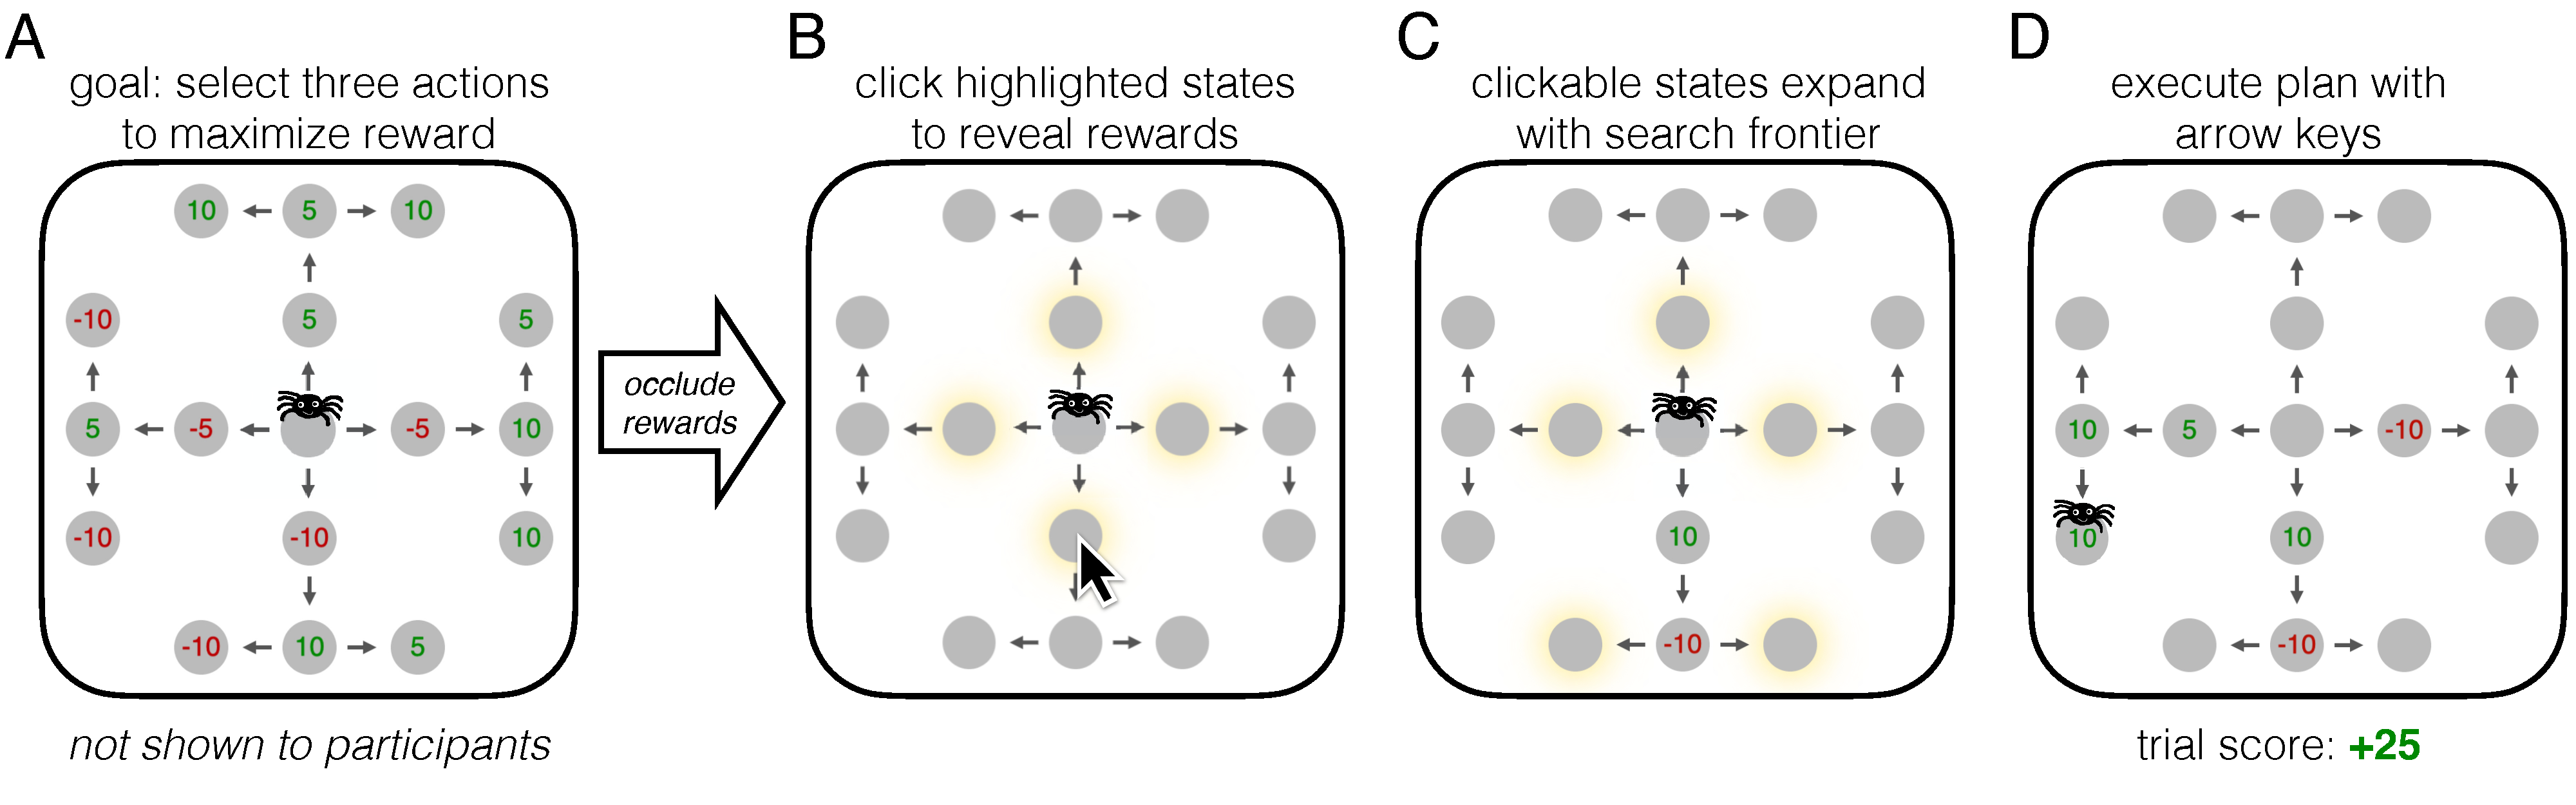
\includegraphics[width=\textwidth]{figs/planning/fig2.pdf}
    \caption{\captiontitle{Experimental task.}
    \subcap{A} Participants are presented with a sequential decision problem displayed as a graph. Gray circles indicate states, arrows indicate actions, and green and red numbers indicate rewards and punishments.
    \subcap{B} Rewards are initially occluded, but can be revealed by clicking on the corresponding state. Only highlighted states can be clicked.
    \subcap{C} The clickable states expand with the search frontier, which includes all states adjacent to either the initial state or an already-clicked state.
    \subcap{D} At any point, participants can execute a plan by pressing a sequence of three arrow keys.}
    \label{fig:planning-task}
\end{figure}

\section{Results}\label{sec:planning-results}

All the models we consider make precise predictions about the exact sequence of node expansion operations a person will execute while planning. The ideal way to test these predictions would be to compare them directly to the node expansion operations performed by people. Unfortunately, this is impossible because those operations are internal and unobservable. Early work on human planning addressed this challenge using ``think aloud'' protocols in which participants narrate their planning process \citep{degroot1965thought,newell1972human,chase1973perception}. However, verbal reports are only indirectly related to the cognitive operations involved in planning and do not lend themselves well to precise quantitative modeling. More recently, researchers have tried to infer people's planning algorithms based only on their external actions \citep{huys2012bonsai,huys2015interplay,daw2005uncertaintybased,solway2015evidence,snider2015prospective,vanopheusden2017computational}. However, the precise nature of a person's planning algorithm is generally only weakly constrained by their actions alone, because there are usually many sequences of planning operations that are consistent with each possible choice. 

How can we collect fine-grained and precise data on human planning processes? A similar problem faced researchers studying how people make non-sequential decisions. To address this challenge, Payne and colleagues developed the Mouselab paradigm \citep{payne1976task,payne1988adaptive}, which traces participants' decision-making processes by requiring them to click to reveal decision-relevant information. In the original paradigm, participants clicked on cells in a table to reveal the payoffs associated with different outcomes of risky gambles. Here, we apply the same idea to multi-step decision problems, with participants clicking to reveal rewards at hypothetical future states.

\subsection{Mouselab-MDP}\label{sec:planning-task}

In order to directly compare our model predictions with human behavior, we developed a task, ``Mouselab-MDP'', which makes human planning observable. The task is illustrated in \figref{fig:planning-task}{}. On each trial, participants are presented with a route-planning problem, displayed as a graph. Each vertex in the graph (gray circles) corresponds to a future state the participant could visit, and harbors a reward or punishment ($-10$, $-5$, $+5$, or $+10$ with equal probability). The edges in the graph correspond to actions the participant can take to travel between states. The goal is to select a sequence of three actions that maximize the total reward. The potential gains and losses are initially occluded, but the participant can reveal them by clicking on the corresponding state, with the constraint that they can only click on states adjacent to the initial state or a previously revealed state. This constraint ensures that participants follow a forward-planning strategy, as has often been assumed in the literature \citep{huys2015interplay,huys2012bonsai,vanopheusden2017computational,macgregor2001information,keramati2016adaptive,krusche2018adaptive,snider2015prospective}; we remove the constraint in Experiment~3. Each click was followed by a three-second delay.

Importantly, the task involves two types of sequential decision problems, both of which can be modeled as MDPs. The problem of moving the spider in the web is modeled as an MDP with $17$ states (gray circles), four actions (key presses), and four possible rewards ($-10$, $-5$, $+5$, and $+10$). In contrast, the problem of selecting which potential rewards to consider when planning a route is modeled as a \emph{metalevel} MDP, with over four billion possible states (patterns of revealed rewards), $16$ actions (one for revealing each reward), and fourteen possible rewards (one implicit cost for the delay and thirteen possible path values, i.e., $-30$ to $30$ in steps of $5$).

\label{predecessor}
Like its predecessor, Mouselab-MDP externalizes the core representations and operations underlying a cognitive process. In particular, our paradigm externalizes the decision tree as the graphical display, the node expansion operation as clicking, and the cognitive cost of that operation as the delay. While it is possible that externalizing a cognitive process in this way might alter the strategy people adopt, the extensive use of the original Mouselab paradigm \citep{payne1988adaptive,ford1989process,payne1993adaptive,gabaix2006costly,schulte-mecklenbeck2011visiting} and the early advances made possible by a less structured form of process tracing \citep{degroot1965thought,newell1972human,chase1973perception} provide support for using this approach. We return to this point in the Discussion.

% \footnotetext{To be more precise, the clicks externalize two components of node expansion: the estimation of the reward to be gained the target state (e.g., by memory recall or simulation), and the expansion of the search frontier. We do not measure (nor explicitly model) the computation of path values, nor the process that selects/updates the currently best path.}


\begin{figure}[t!]
  \centering
  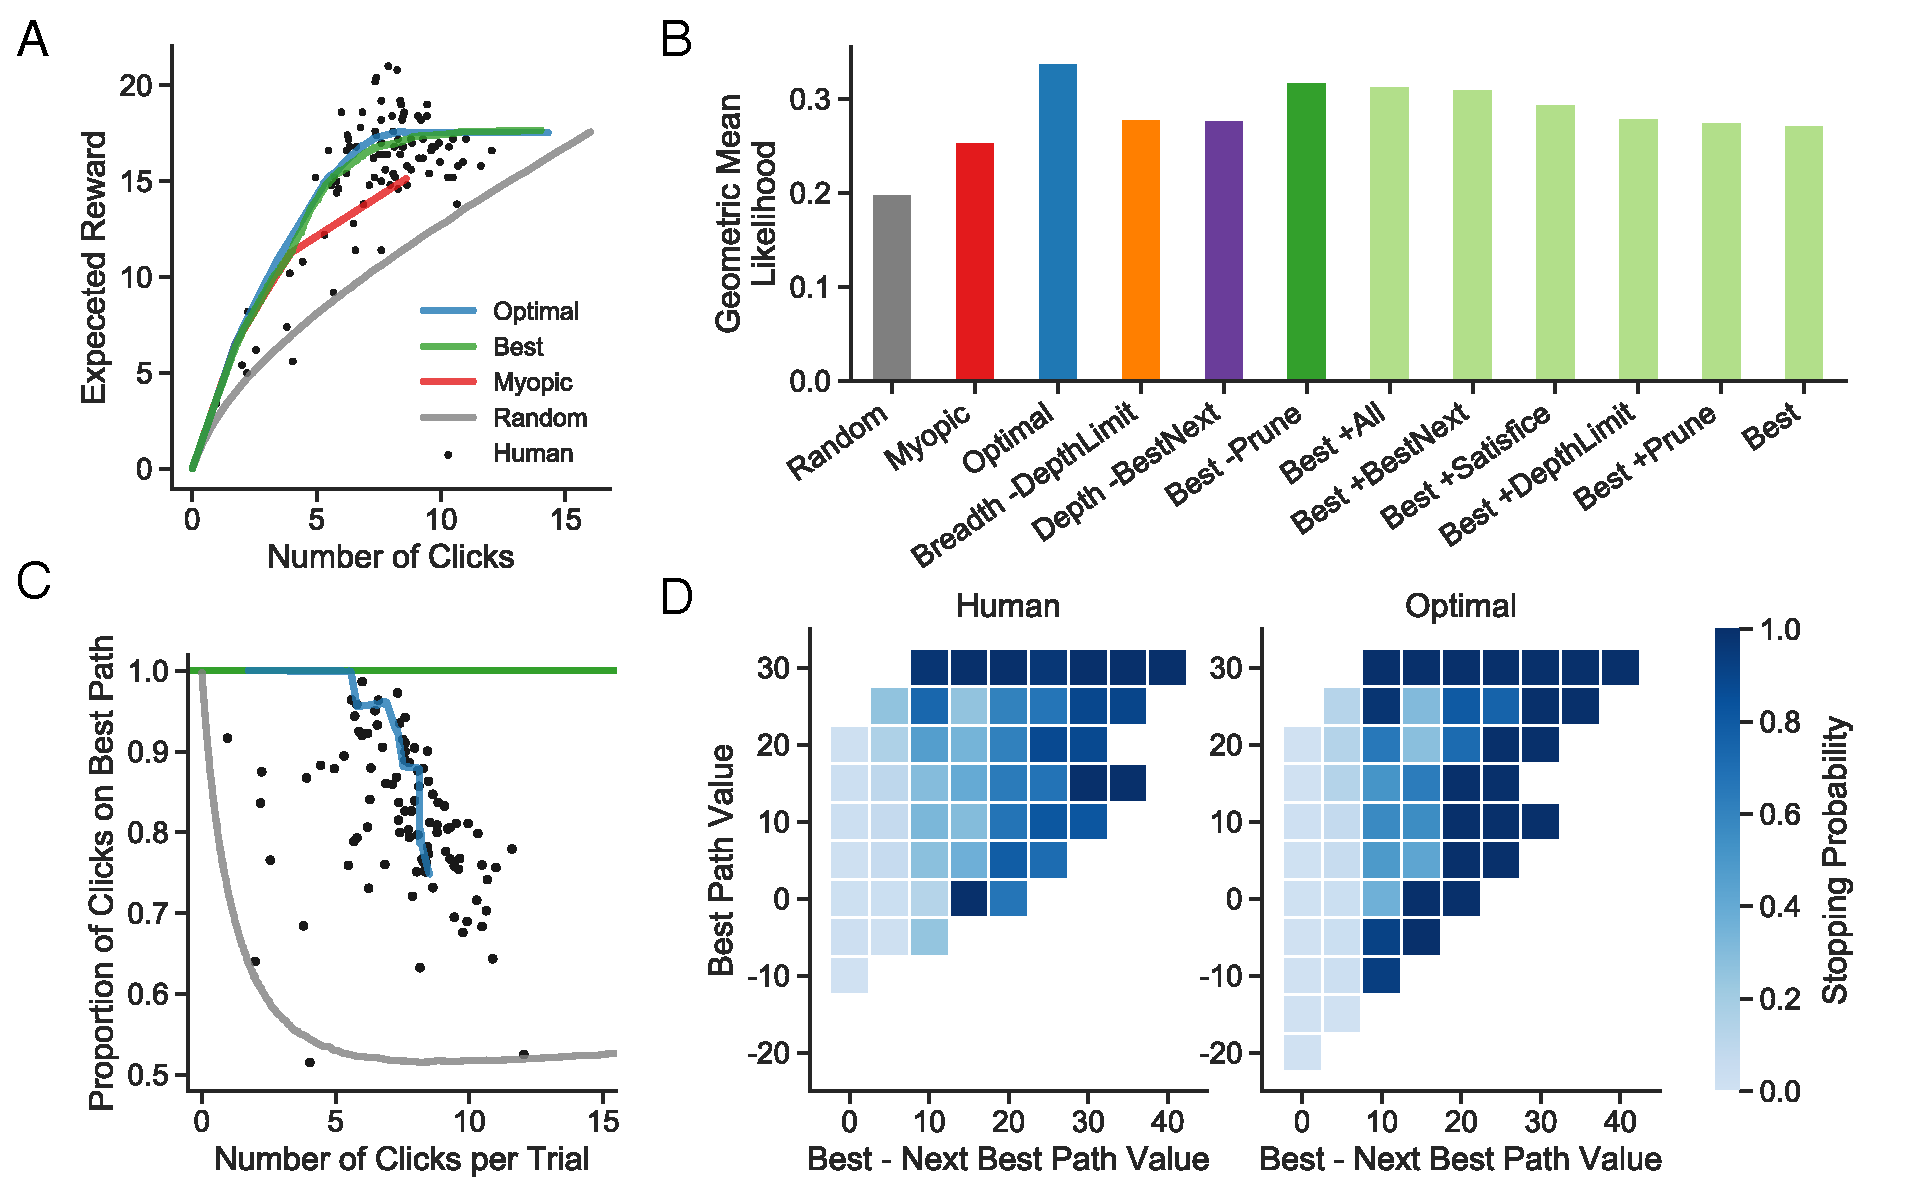
\includegraphics[width=\textwidth]{figs/planning/fig3.pdf}
  \caption{\captiontitle{Experiment~1 results.}
    \subcap{A} Pareto curves. Each point shows the average reward attained and number of clicks made by a participant (black dots) or model (colored lines). Note that with a small number of trials, it is possible to exceed the expected performance of the optimal model by getting lucky.
    \subcap{B} Model comparison. Bars show geometric mean likelihood (the total log-likelihood divided by the number of observations and then exponentiated) estimated on out-of-sample data. For the heuristic models, we indicate which heuristic components are present: +All indicates that all mechanisms are included, -Prune indicates that all mechanisms except for pruning are included. The best-fitting versions each heuristic model are shown in dark bars. Alternative best-first search models are shown in light green. Note that any visually detectable difference corresponds to a large difference in likelihood.
    \subcap{C} Selection rule. Proportion of clicks following a best-first strategy as a function of the average number of clicks per trial for each participant. Colors match panels A and B. Model predictions are made without fitted noise parameters.
    \subcap{D} Stopping rule. Probability that planning is terminated as a function of the value of the best path found yet and the difference in values of the best and next best paths. The right panel shows simulations from the noise-free optimal model. Cases in which all nodes have been clicked and termination is required are excluded.
  }
  \label{fig:planning-exp1}
\end{figure}


\subsection{Experiment~1: Comparing human and optimal planning algorithms}\label{sec:planning-results1}

In our first experiment, we sought to test the extent to which human planning is consistent with an optimal planning strategy in a relatively unstructured environment, illustrated in \figref{fig:planning-task}{a}.

\subsubsection{Overall performance}\label{sec:planning-overall}

To evaluate participants' performance, we must consider both the scores they achieved as well as the amount of planning effort (i.e., clicking) that they expended. \figref{fig:planning-exp1}{a} thus shows the average reward and number of clicks each participant made per trial. The blue line shows the Pareto front, the maximum average reward attainable for a given average number of clicks. On average, participants earned $0.92$ fewer points than they could have with the same number of clicks. They earned $4.94$ more than clicking randomly ($95\%$ CI [$4.43$, $5.44$]; Wilcoxon test: $z = 8.40, p < .001$). Confidence intervals are boot-strapped over participants and p-values are two-tailed (see Section~\ref{sec:planning-stats}).

\subsubsection{Selection rule: cost-dependent best-first}\label{sec:planning-selection}
We first considered the order in which the model expands nodes. Inspecting simulations of the optimal planning strategy across a range of costs ($0.05$ to $3.75$, the maximum cost for which any planning occurs), we found that the optimal model expands a node on a path that has maximal expected value between $74.6\%$ and $100\%$ of the time, compared to $51.7\%$ in the random clicking model.
That is, optimal planning in this environment resembles best-first search. Consistent with this prediction, participants expanded a path with maximal expected value on average $81.5\%$ of the time ($95\%$ CI [$79.6$, $83.3$]; Wilcoxon test vs. chance: $z = 8.46, p < .001$).
% and 100\% of the time, compared to 51.7\% in the random clicking model.

However, the degree to which optimal planning conforms to best-first search depends on the cost parameter, with a closer match for higher costs.
Intuitively, this is because the optimal planning policy expands nodes that are likely to lead to a quick decision. When the cost is high, a plan can be chosen when it is only moderately better than its competitors; the path that currently has maximal value is the most likely candidate. When the cost is low, however, a plan must be exceptionally good to justify stopping early; a path with moderately high value is actually less likely to provide such an outcome, compared to a completely unexplored path.
As a result, the optimal model predicts that the degree to which people follow best-first search will decrease with the average number of clicks they make (the most direct behavioral correlate of the cost parameter). \figref{fig:planning-exp1}{c} confirms this prediction (Spearman's $\rho=-0.481$, $95\%$ CI [$-0.66$, $-0.28$], $p < .001$). The correlation also arises in the random model because all paths are ``best'' on the first click. However, controlling for the best-first rate of the random model, we still find a significant correlation ($\rho=-0.347$, $95\%$ CI [$-0.56$, $-0.12$], $p < .001$).
% and 100\% of the time, compared to 51.7\% in the random clicking model.
% However, we still find a significant correlation in the chance-corrected best-first rate ($\rho=-0.347$, $95\%$ CI [$-0.56$, $-0.12$], $p < .001$).

\subsubsection{Stopping rule: both absolute and relative}\label{sec:planning-stopping}
By inspecting simulations of the optimal model with a range of costs matching that inferred from human participants, we found that the model was more likely to stop planning when it had found a path with high expected value, consistent with satisficing. However, its stopping decisions were more strongly influenced by the difference between the value of the best path and the next best path. That is, the optimal stopping rule depends primarily on the best path's relative value, but also on its absolute value.

As illustrated in \figref{fig:planning-exp1}{d}, our participants' decisions to terminate planning were also sensitive to both the absolute and relative value of the best path. A mixed-effects logistic regression with random intercepts and slopes for each participant revealed significant effects of both terms (best path value: $\beta = 0.82$, $95\%$ CI [$0.69$, $0.94$], $z = 12.89$, $p < .001$; best vs. next: $\beta = 1.68$, $95\%$ CI [$1.52$, $1.84$], $z = 20.70$, $p < .001$). However, compared to the coefficients for the optimal model ($\beta = 0.99$, $95\%$ CI [$0.84$, $1.15$] and $\beta = 4.64$, $95\%$ CI [$4.02$, $5.26$]), people appear to be under-sensitive to relative value (note that the confidence intervals for the optimal model are not negligible due to the mixed-effects structure; predictors are standardized by their mean and SD in the human data).
% However, we still find a significant correlation in the chance-corrected best-first rate ($\rho=-0.347$, $95\%$ CI [$-0.56$, $-0.12$], $p < .001$).

These results are broadly consistent with evidence accumulation models of non-sequential decisions, where relative stopping rules (specifically best vs. next) generally perform better, both in terms of fitting data \citep{ratcliff2004comparison,teodorescu2013disentangling} and maximizing accuracy \citep{mcmillen2006dynamics,bogacz2006physics}. However, although both the model's and our participants' stopping decisions were primarily driven by relative value, absolute value also played a role. This raises the intriguing possibility that people could be using a hybrid stopping rule in simple value-based choices as well.

\subsubsection{Model comparison}\label{sec:planning-comparison}
Having characterized the qualitative matches and mismatches between participant and optimal behavior in the task, we next sought to quantify the ability of the optimal and heuristic models to predict human behavior quantitatively.
%
We fit our models to participants at the individual level and obtained out-of-sample predictions using five-fold cross-validation. We used the total log-likelihood (LL) across all five folds as a measure of model performance. Note that this metric accounts for the flexibility of the different models without relying on parameter counting (as do AIC and BIC), which can be a poor measure of flexibility \citep{piantadosi2018one}. Differences in this cross-validated log-likelihood ($\dnll$) can be interpreted similarly to differences in AIC: $\dnll = 1$ is roughly equivalent to $\Delta_{\mathrm{AIC}} = 2$.

\figref{fig:planning-exp1}{b} shows the predictive accuracy achieved by each of the models. The optimal model clearly outperforms the random, myopic, breadth-first, and depth-first models (all $\dnll > 3981$). In terms of total likelihood, it also outperformed best-first search (all $\dnll > 1250$), although $41$ participants were best fit by the one of the best-first models vs. $45$ by the optimal model ($9$ by some other model). Importantly, given that the best-first model achieved a near-optimal reward-effort trade-off (\figref{fig:planning-exp1}{a}), a substantial majority of participants were best fit by an optimal or near-optimal model.
%



\begin{figure}[p]
  \centering
  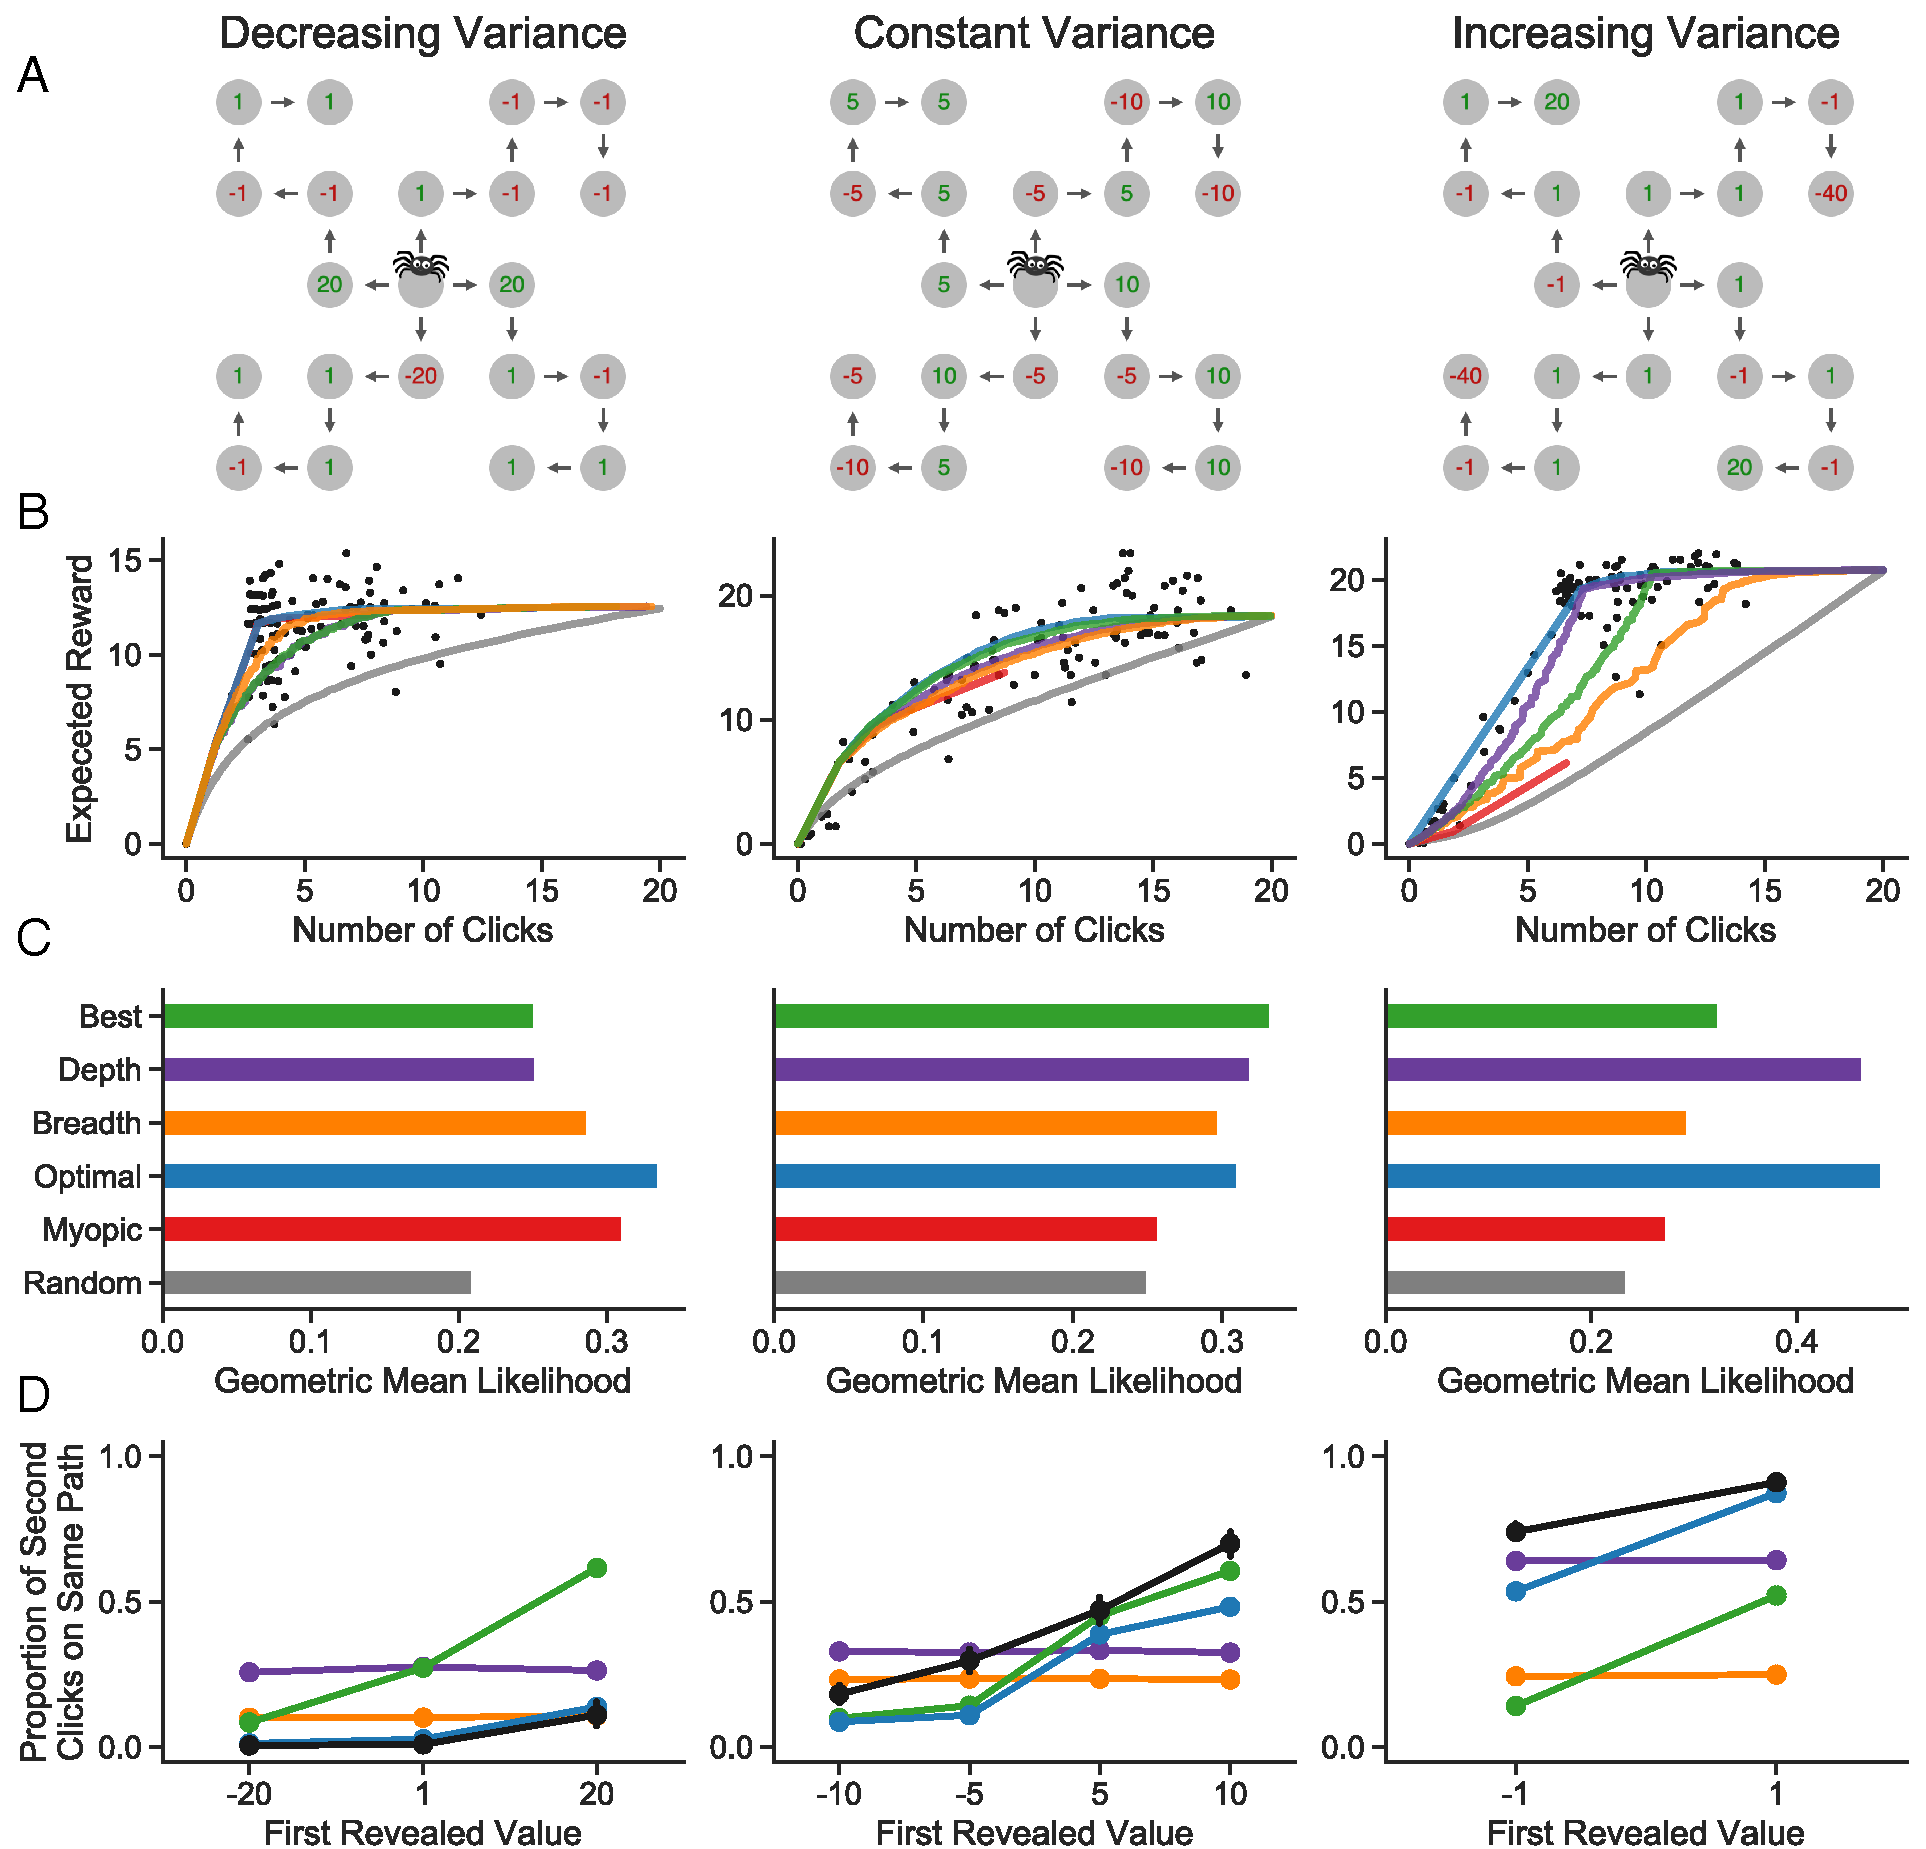
\includegraphics[width=\textwidth]{figs/planning/fig4.pdf}
  \caption{\captiontitle{Experiment~2 results.}
    Each column shows one experimental condition.
    \subcap{A} Example trials. Large values are found at the beginning of each path (decreasing variance), at any location (constant variance), or at the end of each path (increasing variance).
    \subcap{B} Pareto curves. Each point shows the average reward attained and number of clicks made by a participant (black dots) or model (colors match panel C). % In each condition one classical algorithm achieves near optimal performance.
    \subcap{C} Model comparison. Best, Depth, and Breadth refer to the versions of the model that performed best in Experiment~1 (excluding depth limits to prevent other Best and Depth from mimicking Breadth). Of these classical algorithms, the one that achieves the best reward-click trade off (shown in panel B) also best predicts human behavior.
    \subcap{D} Behavioral indicator of planning strategy. Each panel shows the probability of making a second click on the same path as the first, depending on the value revealed by that first click. In each condition, one heuristic model captures the behavioral pattern, but only the optimal model captures the behavior in all conditions.
    Human data is in black and model colors match panel C. All heuristic mechanisms are excluded (see \figref{fig:second_click_alt}{} for the full models). For human data, points show means and error bars show bootstrapped 95\% confidence intervals, both computed across participants.
  }
  \label{fig:planning-exp2}
\end{figure}



\subsection{Experiment~2: Adapting to the environment}\label{sec:planning-results2}
In Experiment~1, we found that participants seemed to use a best-first search strategy that was well-suited to the task environment. However, this does not mean that people always plan in this way. 
On the contrary, a key prediction of the optimal model is that people adapt their strategy to the structure of the environment. We tested this prediction in Experiment~2.

To investigate the effect of environment structure on human planning strategies, we constructed three new experimental environments (see \figref{fig:planning-exp2}{a}). The environments have the same transition structure (four independent paths with five steps each) but different reward distributions. In the ``constant variance'' environment all states had the same reward distribution, as in Experiment~1. In the other two environments, most states had low variance; extreme rewards could only be found in one state on each path. In the ``decreasing variance'' environment extreme rewards were possible only in the first state on each path. In the ``increasing variance'' environment extreme rewards were possible only in the last state.

We designed these environments to produce clear qualitative differences in the predictions of the optimal model. Specifically, in each environment, the optimal planning strategy resembles a different classical planning algorithm: breadth-first for decreasing variance, best-first for constant variance, and depth-first for increasing variance. As illustrated in \figref{fig:planning-exp2}{b}, each algorithm is approximately optimal in its respective environment, but suboptimal in the other two.

If people indeed adapt their planning strategy to the environment, we should find that, out of these three classical search models, the model that achieves the best reward-effort trade-off should also predict human behavior best. \figref{fig:planning-exp2}{c} confirms this prediction (all $\dnll > 446$). For the classical search models, we used the combination of heuristic mechanisms that achieved the best likelihood across all conditions; however, we excluded depth limits from this analysis because they allow the best-first and depth-first models to mimic breadth-first search. With the unrestricted set of heuristic models, the optimal model best predicts human behavior in the increasing ($\dnll = 606$) and decreasing ($\dnll = 1276$) conditions; the best-first model with best vs. next fits best in the constant condition (compared to optimal: $\dnll = 2150$).

\figref{fig:planning-exp2}{d} demonstrates the shift in planning strategy with a simple behavioral measure. Considering only trials on which at least two clicks were made, we can ask how often people use their second click to continue down the path that they began with their first, depending on the value revealed by that first click. An overall tendency to continue down the same path is consistent with a depth-first strategy, the reverse tendency is consistent with a breadth-first strategy, and high sensitivity to the revealed value is consistent with a best-first strategy; we illustrate this by plotting the predictions of the basic search models without any heuristic mechanisms. Participants in each condition show the same pattern as the adaptive search order.

\begin{figure}[p]
  \centering
  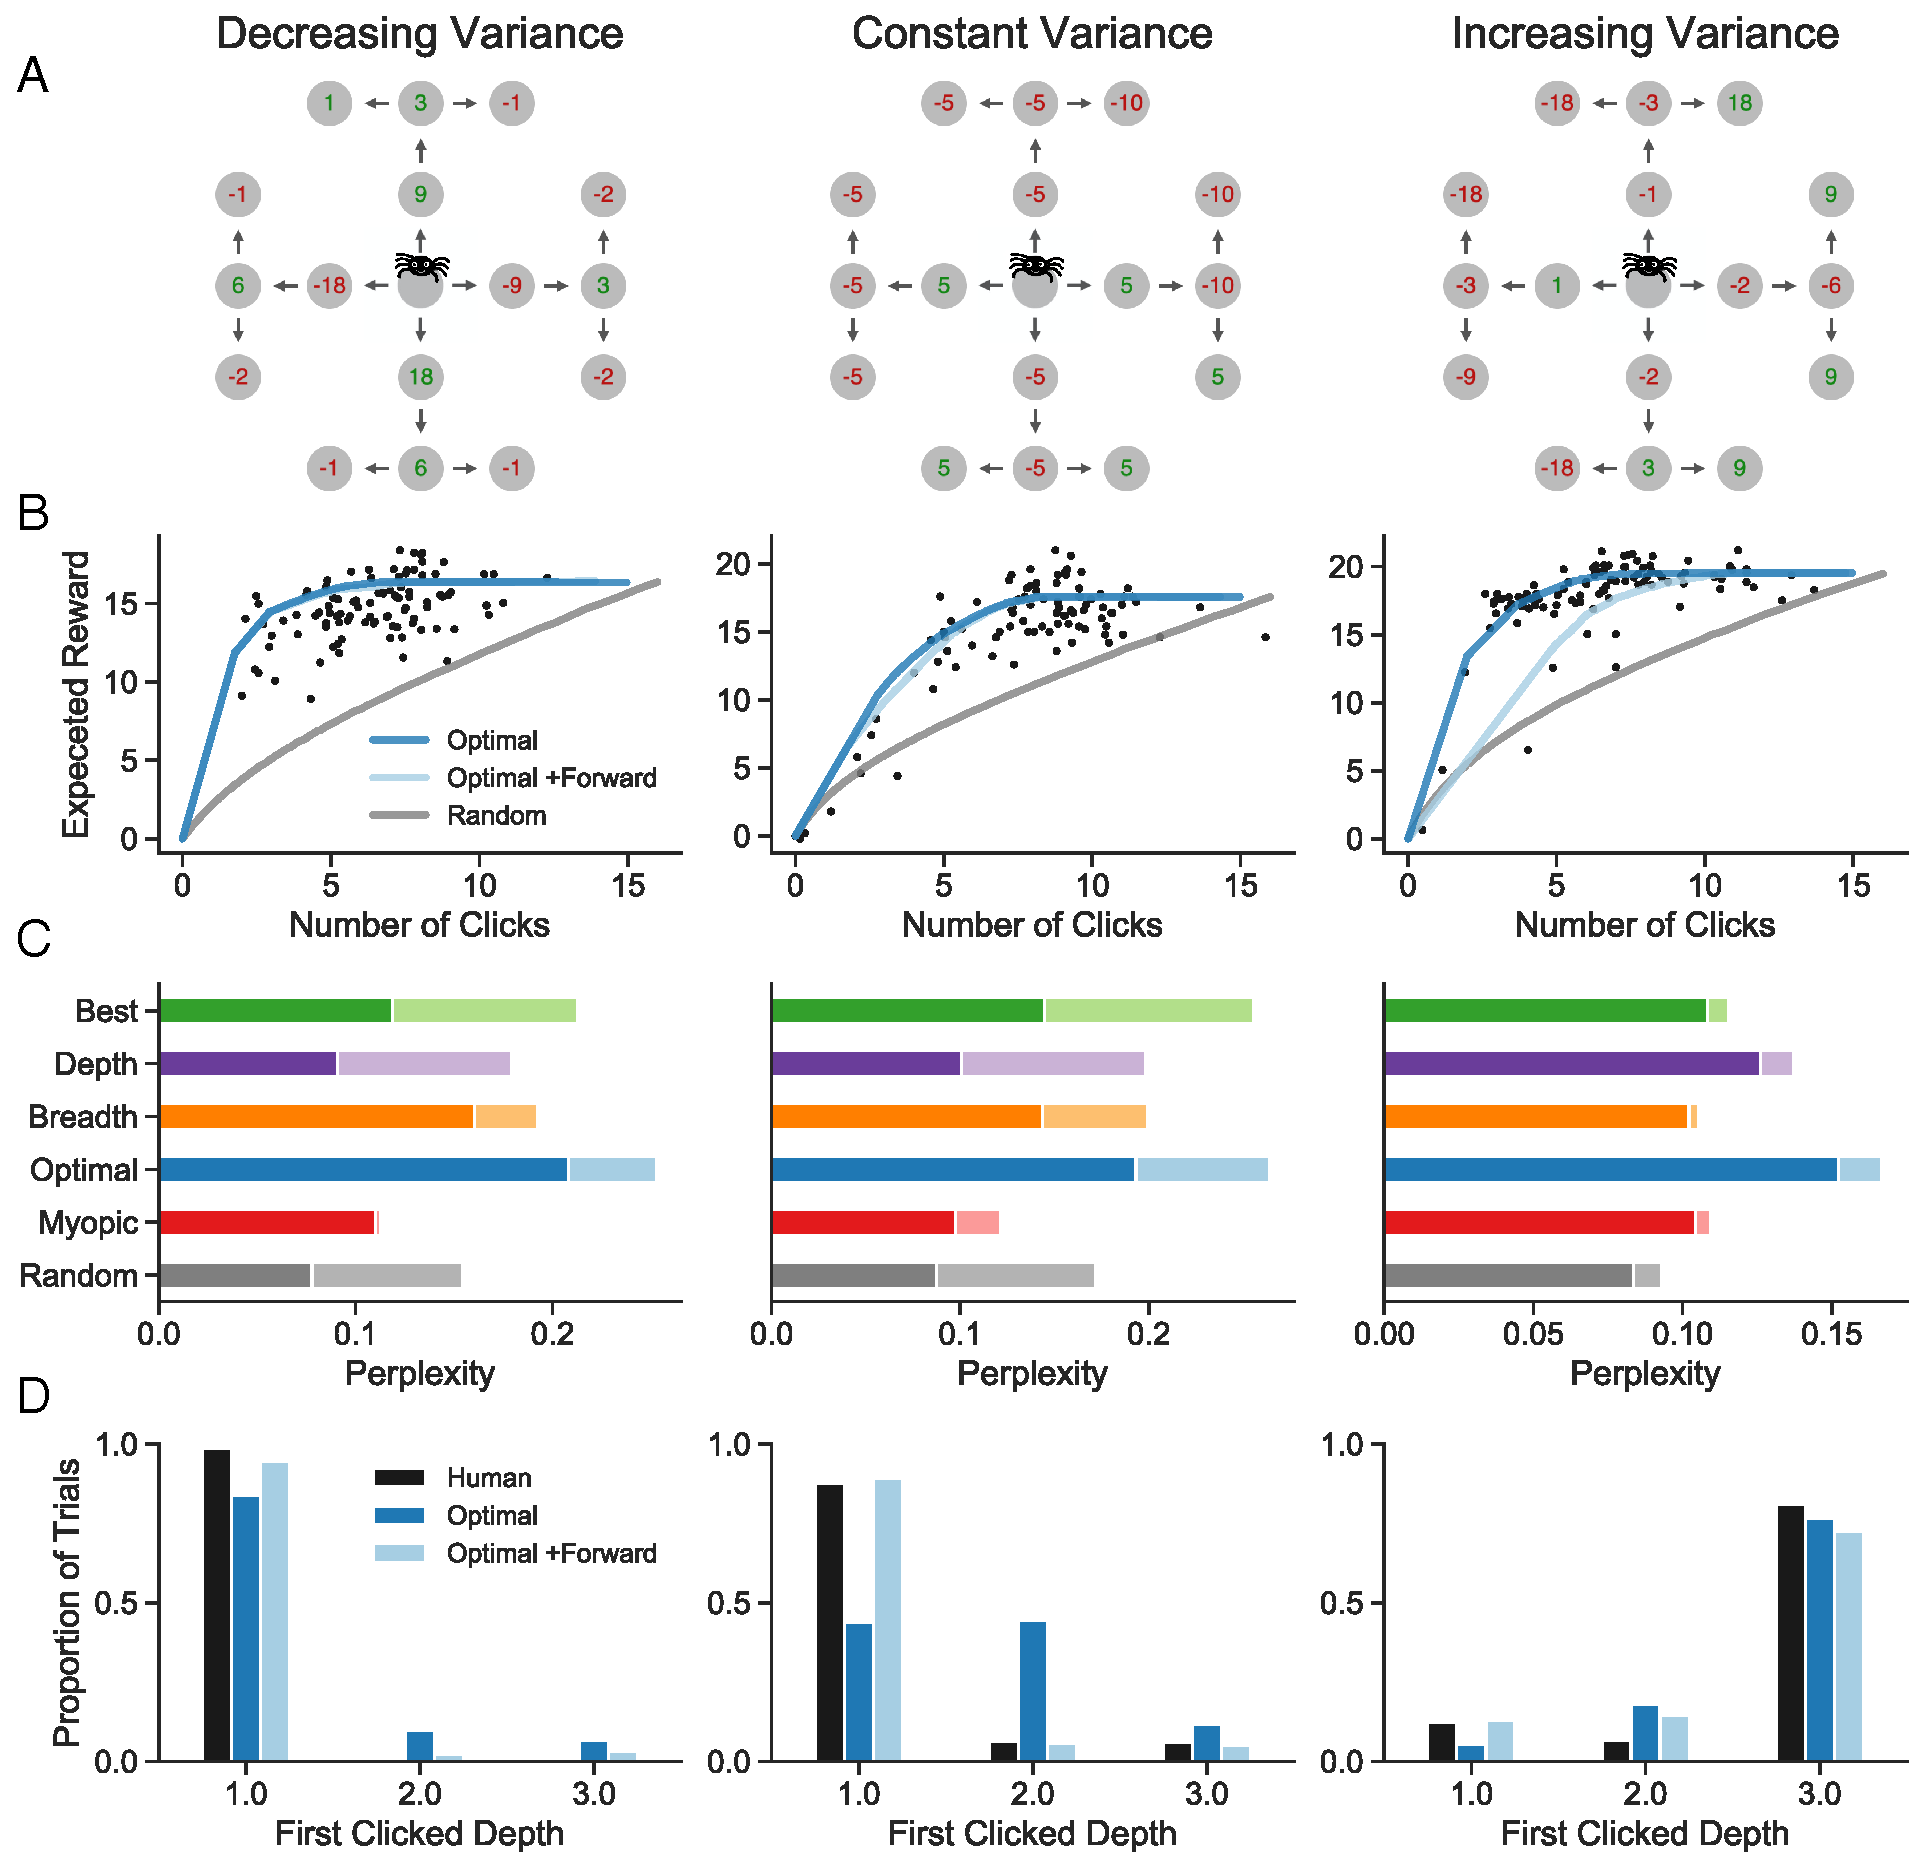
\includegraphics[width=\textwidth]{figs/planning/fig5.pdf}
  \caption{\captiontitle{Experiment~3 results.}
  \subcap{A} Example trials. Each condition is characterized by a different location-dependent reward distribution with standard deviation linearly increasing, decreasing, or remaining constant with depth.
  \subcap{B} Pareto curves. 
  The light blue line shows the optimal model restricted to plan forwards.
  \subcap{C} Model comparison. Light bars show the performance of the corresponding model with a fitted degree of forward-search bias (including the no-bias model and forward-only model as special cases).
  \subcap{D} Behavioral indicator of forward and backward planning. Each panel shows a histogram of the depth of the first clicked state, in the data and in simulations from the optimal model with and without a forward-search bias. Although participants use forward-search by default (center), they switch to backward search when the environment encourages this strategy (right).
  \vspace{1cm}
  }
  \label{fig:planning-exp3}
\end{figure}


\subsection{Experiment~3: Backwards planning}\label{sec:planning-results3}
In the previous experiments, we constrained participants' planning strategies to variations of decision tree search by only allowing them to click on states adjacent to the initial state or a previously-clicked state. However, people may sometimes use planning strategies that are not constrained in this way. For example, they may plan backward from a goal as in means-ends analysis \citep{newell1972human} or they may even consider states in arbitrary order \citep{sutton1990integrated}. Experiment~3 thus investigated a broader class of possible planning algorithms by lifting the forward-planning constraint, allowing participants to click any state at any point.

As in Experiment~2, we used environments with decreasing, constant, and increasing variance. For this experiment, we employed the transition structure from Experiment~1 and decreased or increased the reward variance exponentially with depth. The constant variance condition used the same reward distribution as Experiment~1. See \figref{fig:planning-exp3}{a} for examples.

The key prediction of the optimal model is that participants will adopt a backward-planning strategy in the increasing variance condition, considering terminal states first and then working towards the initial state. Consistent with this prediction, participants in this condition were most likely to click a terminal state first (\figref{fig:planning-exp3}{d}, right).

However, we also see a systematic deviation from the optimal model predictions. In the constant variance case (\figref{fig:planning-exp3}{d}, center), the model is completely neutral between depth-one and depth-two states because they provide equivalent information about the optimal path. In contrast, participants showed a strong tendency to click a depth-one state first. More generally, participants in the constant-variance condition showed a consistent bias for forward search, clicking a state whose parent had already been revealed $92.4\%$ of the time compared to $75.5\%$ in the noise-free optimal model simulations ($95\%$ CI [$86.2$, $94.4$], Wilcoxon test vs. optimal $z = 5.32, p < .001$). Importantly, however, such a bias was not maladaptive as indicated by the strong performance of a strictly-forward planning strategy (\figref{fig:planning-exp3}{b} center).

\figref{fig:planning-exp3}{b} shows that augmenting the models with a forward-search bias improves predictive accuracy considerably. Whether or not we incorporate the bias, the optimal model predicted human behavior best in every condition (with bias: all $\dnll > 509$). Note that it is not clear how to extend pruning and depth limits when non-adjacent nodes on a single path can be expanded; thus, we do not include these mechanisms for this analysis.


\begin{figure}[t!]
  \centering
  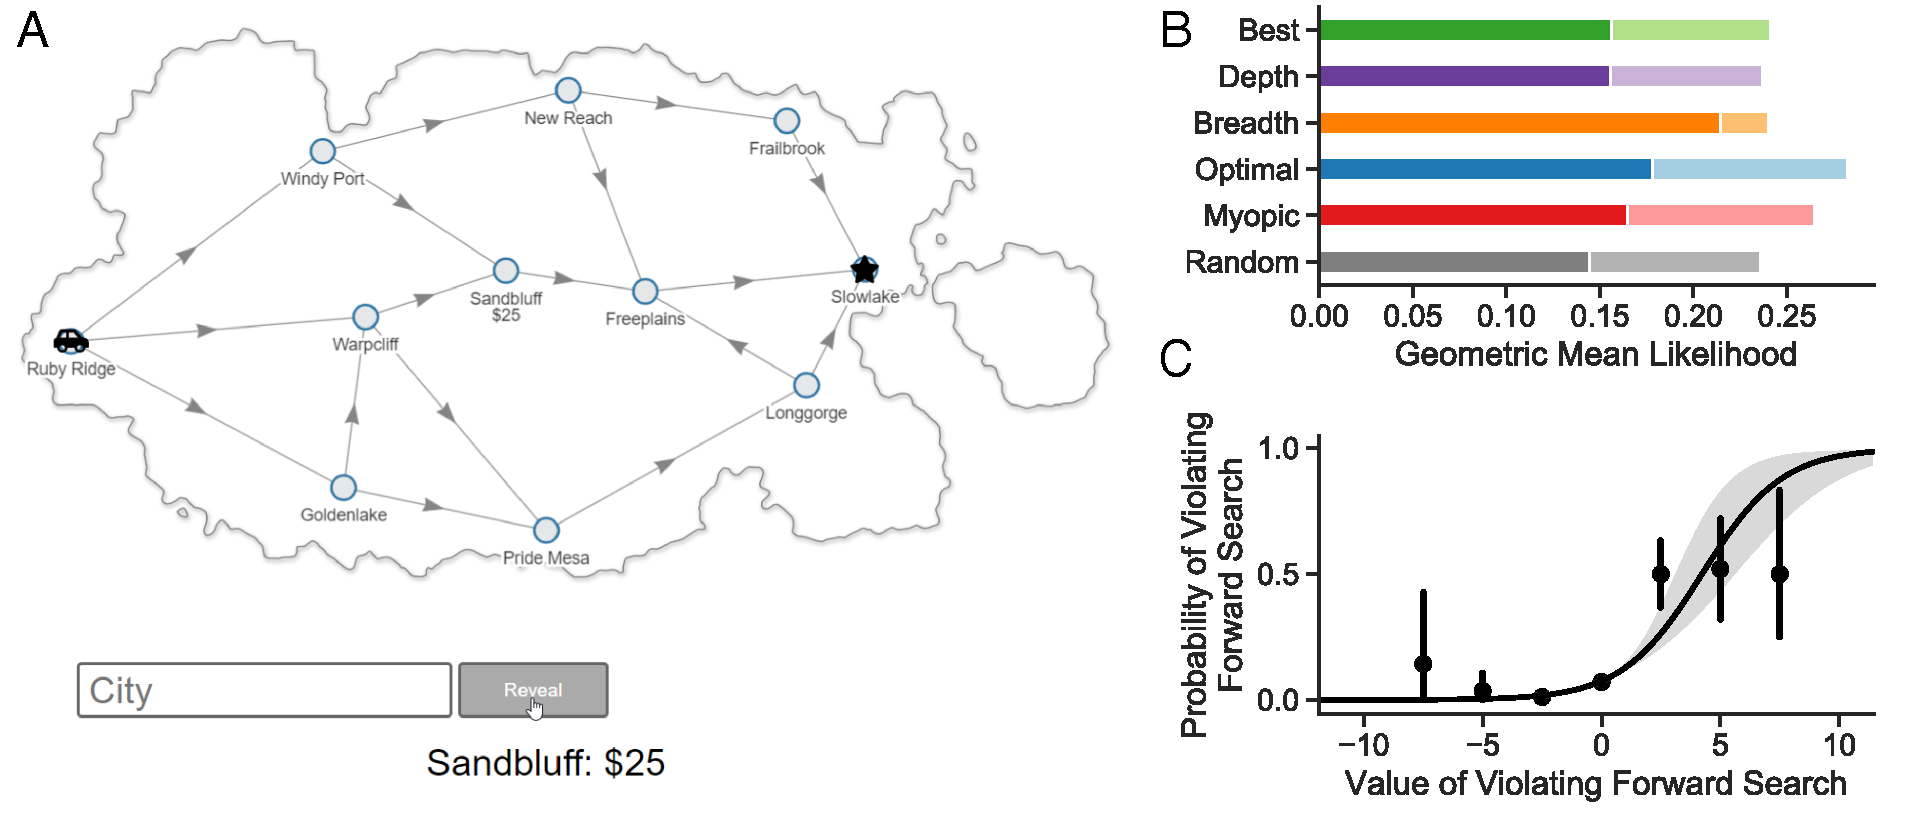
\includegraphics[width=\textwidth]{figs/planning/fig6.pdf}
  \caption{\captiontitle{Experiment~4 results.} 
    \subcap{A} Task: participants acted as a travel agent, attempting to find a low-cost route from a start city to a goal city. They could reveal the price of passing through each city using a textual search interface.
    \subcap{B} Model comparison. Light bars show models augmented with a forward-search bias.
    \subcap{C} The probability of a participant inspecting a city without a revealed parent (i.e., violating forward search) as a function of the value of doing so. This value is defined as the maximal Q value for expanding a node not on the frontier minus the maximal Q value for expanding a node on the frontier. The line shows a logistic regression fit and points show binned means. The shaded regions and error bars show 95\% confidence intervals.
  }
  \label{fig:planning-exp4}
\end{figure}


\subsection{Experiment~4: Planning a road trip}\label{sec:planning-results4}

In Experiment~4, we tested the ability of the optimal model to generalize to a new task environment. In this new task, illustrated in \figref{fig:planning-exp4}{a}, participants acted as travel agents, planning a route from an initial city to a goal city and minimizing the price of hotels that must be visited along the way. Participants were informed that hotels could cost $\$25$, $\$35$, $\$50$, or $\$100$ (with equal probability), but to see the actual price of the hotel in a city they had to type its name into a search box.

Although the task has the same formal structure as that used in Experiment~3 (allowing us to use the same models), there are three important dimensions on which the new task differs from the previous ones. First, rather than allowing participants to plan an arbitrary path, they were required to reach a specific destination; second, the transition structures were not limited to trees---that is, there could be multiple ways to reach a given state; third, the distribution of possible costs did not have a mean of zero, making it necessary to account for expected future cost when estimating the value of an incomplete plan. This task thus provides a non-trivial test of the model's ability to generalize.

As illustrated in \figref{fig:planning-exp4}{b}, the optimal model most accurately predicted human behavior when the bias for forward search was taken into account ($\dnll = 295$). Interestingly, the forward search bias is so important for capturing behavior that when we remove it, the breadth-first model (which follows forward search by default) performs best. 

However, the tendency towards forward search was not without exception. Participants violated forward search by looking up a city without a revealed parent $7.2\%$ of the time. \figref{fig:planning-exp4}{c} shows that these exceptions were not random: participants were more likely to violate forward search when doing so was more valuable (logistic regression with random slopes and intercepts for each participant: $\beta = 2.48$, $95\%$ CI [$1.59$, $3.37$], $z = 5.48$, $p < .001$).

\section{Discussion}\label{sec:planning-discussion}

In this paper, we proposed a rational model of resource-constrained planning and compared the predictions of the model to human behavior in a new process-tracing paradigm. Our results suggest that human planning strategies are highly adaptive in ways that previous models cannot capture. In Experiment~1, we found that the optimal planning strategy in a generic environment resembled best-first search with a relative stopping rule. Participant behavior was also consistent with such a strategy. However, the optimal planning strategy depends on the structure of the environment. Thus, in Experiments~2 and~3, we constructed six environments in which the optimal strategy resembled different classical search algorithms (best-first, breadth-first, depth-first, and backward search). In each case, participant behavior matched the environment-appropriate algorithm, as the optimal model predicted.

The idea that people use heuristics that are jointly adapted to environmental structure and computational limitations is not new. First popularized by Herbert Simon \citep{simon1955behavioral}, it has more recently been championed in ecological rationality, which generally takes the approach of identifying computationally frugal heuristics that make accurate choices in certain environments \citep{gigerenzer2008why,gigerenzer2011heuristic,todd2003bounding,gigerenzer1996reasoning}. However, while ecological rationality explicitly rejects the notion of optimality \citep{gigerenzer1999simple}, our approach embraces it, identifying heuristics that maximize an objective function that includes both external utility and internal cognitive cost. Supporting our approach, we found that the optimal model explained human planning behavior better than flexible combinations of previously proposed planning heuristics in seven out of the eight environments we considered (see Table~\ref{tab:order}).

Why did the optimal model generally explain human behavior better than the heuristic models? One possibility is that the optimal model has a more sophisticated stopping rule, informed by the full distribution of possible rewards, not just the expected values of different paths. Indeed, augmenting the heuristic models with distributional variants of the best vs. next and satisficing rules improved fit substantially (see Appendix~\ref{app:planning-probstop}). However, the optimal model still achieved a better fit in all but two cases (constant variance in Experiments~2 and~3).

The increasing variance environments in Experiments~2 and~3 provide an especially interesting test of the model. In these environments, distal rewards are more extreme than proximal ones, and so the optimal model considers these states as soon as possible. In contrast, a classic finding is that people tend to neglect long-term consequences \citep{odonoghue1999doing}, suggesting that people might fail to consider those distal states in their planning. We found that people's clicking was consistent with the optimal model. In Experiment~2, they ignored small short-term losses to more quickly find large long-term rewards (\figref{fig:planning-exp2}{d}), and when we lifted the forward-planning constraint in Experiment~3, people considered the final states first (\figref{fig:planning-exp3}{d}). A potential reason why people were more far-sighted in our experiments than they are in some real-world situations is that our experiment allowed them to learn about the structure of the decision environment and adapt their decision strategy to it through intensive practice with immediate, reliable performance feedback that is often unavailable in the real world \citep{kahneman2009conditions}. Consistent with this, people did show a strong bias to consider proximal rewards first when the environment did not strongly incentivize a different strategy (\figref{fig:planning-exp3}{d}, center).

The ways in which our participants deviated from the optimal model are equally---if not more---informative than the ways in which they were consistent \citep{norris2021more}. Using the approach of resource-rational analysis \citep{griffiths2015rational,lieder2020resourcerational}, we can use the observed discrepancies to generate hypotheses about additional constraints (internal or external) that shape human planning strategies. That is, people's cognitive resources might be more limited than the model assumes and they may be adapted to an environment that differs from our artificial experimental task in important ways.

We found the most striking deviation from the optimal model's predictions in Experiments~3 and~4, where we observed a strong bias for forward search when it was not adaptive (nor clearly maladaptive, see \figref{fig:planning-exp3}{b}). 
This suggests that people's default representation of plans is temporally ordered, and that representing or computing information which does not fit this temporal structure is cognitively costly.
There are two reasons such a representation might be preferred.
First, in many (but not all) natural environments, the set of states one could feasibly reach is not clear in advance; one can only discover such states by forward search. In these cases, the standard assumption that people can only search in the forward direction \citep{keramati2016adaptive,vanopheusden2017computational,huys2012bonsai,snider2015prospective} may be appropriate. Second, in many domains, people likely have generative models of the world \citep{battaglia2013simulation,jara-ettinger2016naive}; given such models, one can directly simulate the consequences of an action, but one must infer what action could have led to a given consequence. In these cases, forward search will be less costly than backward search, but still possible; this is consistent with \figref{fig:planning-exp4}{c}.

% One puzzling aspect of our results is that the best-fitting heuristic model in Experiments~1 and 2 did not include pruning. Consistent with the results of Huys and colleagues \citep{huys2012bonsai,huys2015interplay}, we did observe a tendency for people to ignore paths that start with a large negative reward; but in our task, this pattern of behavior was fully accounted for by best-first search. In a more complex task, however, van Opheusden and colleagues \citep{vanopheusden2017computational} found that a combination of best-first search and pruning best explained participant behavior. One possible explanation for this difference is that a key motivation for pruning is to limit the number of possible plans one must hold in working memory (in addition to the number of nodes expanded). Our paradigm removes this working memory constraint, making pruning less useful.

One important limitation of our work is that externalizing planning, as our task does, may alter the internal process that we wish to measure \citep{lohse1996comparison}. Nevertheless, there are at least five reasons to believe that the present results already reveal something important about human planning. First, the paradigm is a direct extension of the Mouselab paradigm, which has been widely used in the multi-attribute and risky-choice literature \citep{payne1988adaptive,ford1989process,payne1993adaptive,gabaix2006costly,schulte-mecklenbeck2011visiting}. Second, our Experiment~1 results replicate previous findings that suggest that participants use a best-first strategy \citep{vanopheusden2017computational}---or, similarly, avoid nodes following large losses \citep{huys2012bonsai}---in the absence of environmental structure that a different algorithm could exploit. Third, we found that people show a bias for forward search even when the task does not require or even encourage it; this suggests that participants are carrying over a strategy that they have developed for naturalistic planning (where such a bias is likely adaptive, as discussed above). Fourth, recent work has noted a parallel between planning and information-seeking (our task could be characterized as the latter), suggesting that similar neural mechanisms may underlie both behaviors \citep{hunt2021formalizing}. Finally, measuring how people plan in the absence of working memory constraints provides a useful comparison point for future work investigating how these constraints shape human planning strategies.

Comparing human and optimal planning in a more naturalistic paradigm is thus a critical step in future research. One promising approach is to use reaction time in a secondary task as a signal of previous planning (e.g., choosing between a subset of actions \citealp{ongchoco2019imagining}, replanning after a random teleportation \citealp{ho2020efficiency}, or determining whether a specific state falls on the optimal path \citealp{solway2014optimal}). Another approach would be to use eye- or mouse-tracking with a display that only reveals the reward at future states, but not the transition function. However, deploying these paradigms would also require augmenting the model to account for constraints on working memory and imperfect knowledge of the transition function---important but challenging directions for future work.

A second limitation of our work is that we only consider deterministic environments. This assumption greatly simplifies the task of identifying optimal strategies; in particular, it ensures that it is optimal to do all planning before taking any actions, allowing us to avoid the complexities associated with interleaving planning and action. Although we enforced this plan-then-act structure in our main experiments, a follow-up experiment (reported in Appendix~\ref{app:planning-experiment5}) found that participants rarely violate this ordering when allowed to do so ($3.9\%$ of trials). However, in stochastic environments, planning far ahead may be wasteful because an unexpected transition can render much of that planning irrelevant. In such cases, it may be optimal to take an action and see its result before planning further ahead (discussed further in Section~\ref{sec:interleaved}). Investigating how people adapt their planning strategies in unpredictable environments is thus an important direction for future work.

A third limitation is that we only consider problems with small, unstructured state spaces. This contrasts with early work exploring human planning in massive state spaces with rich internal structure, such as propositional logic \citep{newell1972human}. Although this limitation applies equally to most recent empirical studies of human planning, future work should explore the strategies people use to plan efficiently in more complex environments.

Taken together, these three limitations put important limits on the conclusions we can draw from our results. Although we have shown that human planning can be quite close to optimal in simple environments without working memory constraints, it remains unclear whether people will be able to plan as effectively in more complex domains when working memory is limited. Nevertheless, our results do suggest that models of efficient use of limited cognitive resources may be a good starting place when developing theories of planning in these more naturalistic conditions.

A final limitation of our work is that we do not provide a process-level theory for how people are able to approximate optimal planning. One plausible hypothesis is that people use a myopic approximation, considering the immediate value of expanding a node while disregarding the potential for future node expansions. Indeed, such an approximation has been employed in two recently proposed models of human planning \citep{mattar2018prioritized,sezener2019optimizing}. However, we found that this model generally performed poorly, both in terms of reward (Figures~\figref[]{fig:planning-exp1}{a} and~\figref[]{fig:planning-exp2}{b}) and predicting human behavior. Another hypothesis is that people learn effective planning strategies through experience \citep{lieder2017strategy,krueger2017enhancing}. However, the mechanisms that allow this learning to proceed so rapidly given the large state spaces of metalevel MDPs are still not well understood.

% \footnotetext{Concretely, the metalevel MDP for Experiment~3 has $5^{16}$ (over 150 billion) states.}

Over the past decades, the assumption that humans are well-adapted to their environment \citep{marr1982vision,anderson1990adaptive} has facilitated rapid progress in many psychological domains \citep{oaksford1994rational,gureckis2012selfdirected,tenenbaum2001generalization,anderson1991adaptive,ashby1995categorization,savage1954foundations}. However, the constraints imposed by the external environment are insufficient to explain many key features of human cognition \citep{rahnev2018suboptimality,lieder2020resourcerational}. By additionally considering the constraints imposed by our limited cognitive resources---that is, our internal environments---we can apply the tools of rational modeling to a much broader set of cognitive phenomena \citep{griffiths2015rational,lieder2020resourcerational}. In this work, we have presented the beginning of such an analysis for planning. We anticipate that more precise characterizations of the cognitive constraints that shape planning will yield a correspondingly deeper understanding of this remarkable human ability.


\section{Methods}\label{sec:planning-methods}

All experiments can be viewed exactly as they were given to participants and in abbreviated form at https://webofcash.netlify.app. All experiments were approved by the institutional review board of Princeton University, and all participants gave informed consent. Each participant could only participate in one experiment (including pilots). For all experiments, we aimed to collect $100$ participants per condition. We did not conduct a formal power analysis because all our hypothesis tests were highly significant in pilot samples. All reported statistics, model comparisons, and figures were pre-registered.\footnote{%
  Experiment~1: \url{https://aspredicted.org/jd8rs.pdf}\par
  Experiment~2: \url{https://aspredicted.org/w4kt2.pdf}\par
  Experiment~3: \url{https://aspredicted.org/2cr5k.pdf}\par
  Experiment~4: \url{https://aspredicted.org/wq87z.pdf}\par
} We describe deviations from the pre-registered analysis plan in Appendix~\ref{app:planning-deviations}.

All data and code supporting this chapter can be found at \url{https://github.com/fredcallaway/rational-resources-planning}.


\subsection{Experiment~1} \label{sec:planning-methods1}
We recruited $104$ participants from Prolific who reported fluency in English, resided in the United States, and had a $95\%$ approval rating (this number excludes participants who accepted the study but did not move past the second instruction page). We excluded $6$ participants because they failed a quiz following the instructions and $3$ participants who did not complete the experiment for some other reason, leaving $95$ participants in the analysis. Participants who completed the experiment or failed the quiz received $\$1.50$ for participation. Those who completed the experiment additionally earned a performance-dependent bonus of (mean $\pm$ sd) $\$2.43$ $\pm$ $\$0.42$ for $22.5$ $\pm$ $6.6$ minutes of work.

\paragraph{Main Task}
In the main task of Experiment~1 (see \figref{fig:planning-task}{}), participants navigated a cartoon spider through a directed graph in which each vertex (the gray circles) harbored a gain or loss, with the goal of maximizing the total payoff accrued along the selected route. All rewards were independently drawn from a discrete uniform distribution over the values $\{-10,-5, +5, +10\}$. At the beginning of each trial, all rewards were occluded; however, participants could click on nodes adjacent to the starting location or to an already-revealed node to reveal the value. After each click, there was a three-second delay during which no additional clicks could be made. To visually convey these constraints, nodes were highlighted whenever they could be clicked. At any point, participants could stop clicking and move the spider from the starting node using the arrow keys. After each arrow key press, the spider moved to an adjacent node, the value of that node was revealed (if not already revealed), and its value was added to a total shown in the top right. Clicking was disabled after the first move, and the trial ended when the participant reached a terminal node (i.e., one with no outgoing edges).


\paragraph{Procedure}
The experiment began with an instruction phase in which participants completed increasingly complex versions of the task. First, they were told the basic goal of selecting paths to maximize the amount of ``money'' acquired, and completed three trials with the rewards fully revealed. Second, they were told the reward distribution and shown ten examples where they did not make choices. Third, they completed one trial with the rewards occluded (i.e., guessing randomly). Fourth, they were told that they could click nodes to reveal the values, and completed three trials in which they had to make at least five clicks. Finally, they were told the conversion between in-game currency and their bonus ($1$ US cent for every $2$ points) and completed three practice trials of the full task.

After completing the instructions, participants took a multiple-choice quiz that asked about the reward distribution, the rules for inspecting nodes, and the points-to-bonus conversion. Participants who failed the quiz were shown a review screen with all the necessary information and were given another chance to complete the quiz. If they failed the quiz three times, they were dismissed. Otherwise, they progressed to the main phase of the experiment where they completed $25$ trials of the main task. They were given an initial endowment of $100$ points to minimize the chance that they would ever have a negative score.

\subsection{Experiment~2}\label{sec:planning-methods2}
All aspects of the design were identical to Experiment~1 except where noted otherwise. We recruited $313$ participants. We excluded $4$ who failed the quiz and $11$ who did not complete the experiment, leaving $298$ participants in the analysis. Participants received $\$1.50$ plus a bonus of $\$2.18$ $\pm$ $\$0.74$ for $23.6$ $\pm$ $10.4$ minutes of work.

\paragraph{Main Task}
The main task of Experiment~2 had the same basic structure as that in Experiment~1, but with a different graph and reward structure (see \figref{fig:planning-exp2}{a}). The graph had a single choice point at the first move (four options) followed by four forced moves. The reward distributions depended on a between-participant condition. In the constant variance condition, it was the same as in Experiment~1. In the other two conditions, most nodes were $-1$ or $+1$ with equal probability, but four nodes had an extreme distribution. For increasing variance, the terminal nodes (farthest from the initial location) had values of $+20$ with $\nicefrac{2}{3}$ probability and $-40$ with $\nicefrac{1}{3}$ probability. For decreasing variance, the nodes closest to the initial location had value $+1$ with $\nicefrac{3}{5}$ probability, and either $+20$ or $-20$ with roughly $\nicefrac{1}{5}$ each, slightly skewed towards $-20$ to make the expected reward $0$ ($.185$ and $.215$). These distributions were selected to make the optimal planning strategy closely resemble depth-first and breadth-first search in the increasing and decreasing variance conditions respectively.

\paragraph{Procedure}
The procedure was identical to Experiment~1 except that we replaced the bonus question with a question asking on which nodes the maximal reward could be found.


\subsection{Experiment~3}\label{sec:planning-methods3}
All aspects of the design are identical to Experiment~2 except where noted otherwise. We recruited $319$ participants. We excluded $11$ who failed the quiz and $17$ who did not complete the experiment, leaving $291$ participants in the analysis. Participants received $\$1.50$ plus a bonus of $\$2.49$ $\pm$ $\$0.43$ for $21.3$ $\pm$ $7.5$ minutes of work.

\paragraph{Main Task}
The task had the same basic structure and graph as Experiment~1. The key difference from previous experiments is that we lifted the restriction that only nodes adjacent to the initial state or already-revealed nodes could be revealed. That is, participants could reveal any unrevealed node at any point. The graph was the same as in Experiment~1. The reward structure varied by condition. In the constant variance condition, it was identical to Experiment~1. In the increasing variance condition, the reward distribution for depth $1$ nodes was uniform over the values $\{-2,-1, +1 +2\}$. The possible values at later depths were scaled by $3^d$; that is, the range and standard deviation increased by a factor of $3$ from each depth to the next, up to $\{-18,-9, +9 +18\}$ at the depth~$3$ leaf nodes. In the decreasing variance condition, the situation was exactly reversed: depth $1$ nodes could take values in $\{-18,-9, +9 +18\}$, and the values decreased by a factor of $3$ with each step down to $\{-2,-1, +1 +2\}$ at the leaf nodes.

\paragraph{Procedure}
The procedure was identical to Experiment~2.


\subsection{Experiment~4}\label{sec:planning-methods4} We recruited $137$ participants from Prolific who reported fluency in English, resided in the United States, and had a $95\%$ approval rating. We excluded $7$ who \ failed the quiz and $37$ who did not complete the experiment, leaving $93$ in the analysis. Due to a technical error, instruction progress was not recorded, hence the larger number of incompletes. Participants received $\$1.75$ plus a bonus of $\$0.99$ $\pm$ $\$0.13$ for $18.2$ $\pm$ $7.8$ minutes of work.

\paragraph{Main Task}
Participants assumed the role of a travel agent planning a road trip. On each trial, the participant saw a map of an island with eleven cities represented as circles and roads represented as arrows. Participants were instructed that the client wants to travel from a given starting location to a goal location. Each ``day'' they can move along any single arrow between two cities and each ``night'' the client has to stay in a hotel at a price that varies between cities. Participants were informed that hotels could cost $\$25$, $\$35$, $\$50$, or $\$100$, and that all values were equally likely. To reveal the price of the hotel in a given city, participants had to type its name into a text box. They could uncover any number of prices, in any order, and they could submit their recommended route at any moment. At this point the total cost was computed; this value was subtracted from a budget of $\$300$ and the participant's bonus for the trial was $1$ cent for each $\$10$ remaining.

\paragraph{Procedure}
The experiment began with an instruction phase in which the task was explained through verbal instructions and images. Participants were required to complete a quiz (in no more than three attempts) before continuing.
Each participant then performed $8$ trials, the first of which was a practice trial that did not count towards their bonus payment.


\subsection{Model specifications}\label{sec:planning-modelspec}
Each of our candidate models corresponds to a parameterized family of metalevel policies. For all models, the policy is specified as a four-step generative process. First, if the frontier is empty (i.e., all nodes have been clicked or pruned), the model executes the termination operation, $\bot$. Second, if the frontier includes at least one node, then a random legal computation is executed with some probability, $\varepsilon$. Otherwise (step~3), the model executes $\bot$ with probability $p\stop^M(m)$; the form of this function depends on the model, $M$. Finally (step~4), if the model did not act randomly or terminate, then it selects a node to expand, each node having probability $p\select^M(m, c)$ The models are thus defined by stochastic stopping and selection rules.

The heuristic models (best-first, depth-first, and breadth-first) all use a common stopping rule that incorporates both the relative and absolute value of the best path identified so far. The stopping probability is a logistic function of a weighted linear combination of these terms, that is,
\begin{equation}\label{eq:stopH}
p\stop^H(m) = \frac{1}{1 + \expp{-f\stop(m)}},
\end{equation}
where
\begin{equation}\label{eq:fstop}
f\stop(m) = 
  \beta\satisfice\cdot V\best +
  \beta_{\mathrm{bestnext}}\cdot (V\best - V\nxt ) +
  \theta\stop.
\end{equation}
$V\best$ and $V\nxt$ are the expected values of the best and second-best paths given the current mental state, $\theta\stop$ sets the midpoint of the logistic function, and the $\beta$'s control the contribution of each term to its slope. This implementation allows the model to both flexibly interpolate between a relative and an absolute stopping rule and also to vary the precision in the application of the rule. For example, a classic ``hard'' satisficing rule can be created by setting $\beta\satisfice$ to a very large number, $\beta_{\mathrm{bestnext}}$ to zero, and $\theta\stop$ to $-\theta \cdot\beta\satisfice$ where $\theta$ is the aspiration level. This results in
\begin{equation}\label{eq:satisfice}
p\stop^\textsc{satisfice}(m) = \frac{1}{1 + \expp{-\beta\satisfice (V\best - \theta)}},
\end{equation}
that is, a logistic function of the expected value of the best path with slope $\beta\satisfice$ and intercept $\theta$.

We defined the selection rule for each heuristic model so that its policy approximates the corresponding classical search algorithm. To do this, we defined
\begin{equation}\label{eq:selectH}
p\select^H(m, c) = \frac{
  \textbf{1}(c \in \frontier(m)) \cdot \expp{\beta\select \cdot f\select^{\textsc{ alg}}(m, c)}
  }{
  \displaystyle\sum_{c' \in \frontier(m)} \expp{\beta\select \cdot f\select^{\textsc{ alg}}(m, c')}
  },
\end{equation}
where $f\select^{\textsc{ alg}}(m, c)$ denotes a node-scoring function for each algorithm; specifically, 
\begin{equation}\label{eq:scoring}
\begin{aligned}
  f\select^{\textsc{\ best}}(m, c^{(i)}) &= V(m, i) = \max_{p \in \lbrace \P \mid i \in p  \rbrace} V(m, p) \\
  f\select^{\textsc{\ depth}}(m, c^{(i)}) &= \mathrm{depth}(i)\\
  f\select^{\textsc{\ breadth}}(m, c^{(i)}) &= -\mathrm{depth}(i).
\end{aligned}
\end{equation}
We chose these node scoring functions to ensure that in the limit $\beta\select\rightarrow\infty$, the model's selection rule is deterministic and exactly matches the corresponding algorithm. Pure best-first search always expands a node with maximal expected value, pure depth-first search always expands the deepest node in the tree, and pure breadth-first search always expands every node at each depth before expanding any at the next depth. However, to account for variability in human selection decisions, we allow for $\beta\select\in [0,\infty)$. 

The random model takes the same form as the heuristic models, with $f\select^{\textsc{ rand}}(m, c) = 0$ and $f\stop(m) = \theta\stop$. This is equivalent to a fixed stopping probability and random selection. In the random model the probability of choosing computations at random is set to zero ($\varepsilon = 0$) because this step is redundant.

For the optimal model, we define both the stopping and the selection rules using the optimal state-action value function, $Q_\gamma$, of the metalevel MDP with computational cost $\gamma$. We computed the $Q$ function using dynamic programming. The stopping rule is
\begin{equation}\label{eq:stopO}
p\stop^O(m) = \frac{ \expp{\beta\stop \cdot Q_\gamma(m,\bot)}}{\displaystyle\sum_{a' \in \frontier(m) \cup \{\bot\}} \expp{\beta\stop  \cdot  Q_\gamma(m, c')}}
\end{equation}
and the selection rule is
\begin{equation}\label{eq:selectO}
p\select^O(m, c) = \frac{\expp{\beta\select  \cdot  Q_\gamma(m, c)}}{\displaystyle\sum_{c' \in \frontier(m)}\expp{\beta\select  \cdot  Q_\gamma(m, c')}}.
\end{equation}
Note that if $\beta\select = \beta\stop$, this corresponds to a single softmax over the full action space. However, we use separate inverse temperature parameters for stopping and selection to match the flexibility of the error model used by the optimal model to that of the heuristic models.

The myopic model has the same form, but the $Q_\gamma$ function is replaced by a myopic one-step approximation \citep{russell1991principles}, which we denote $Q_\gamma\myopic$. For the termination operation, this approximation is exact because the trial ends after this action is executed and thus $Q_\gamma(m, \bot) = Q_\gamma\myopic(m, \bot) = r(m, \bot)$. For expansion, the myopic model approximates the Q value as the expected value of stopping at the next time step (after expanding a node) minus the expansion cost, that is
\begin{equation}
Q_\gamma\myopic(m, c) = \E_{s' \sim T(\cdot \mid m, c)}\left[ 
  r(s', \bot)
\right] - \gamma.
\end{equation}

\subsection{Pruning and depth limits}\label{sec:planning-pruning}
To model pruning \citep{huys2012bonsai,huys2015interplay} and depth limits \citep{keramati2016adaptive,snider2015prospective}, we assume that each time a participant expands a node, she may choose to eliminate the corresponding branch from further consideration. Because both mechanisms ultimately involve removing a branch of the decision tree, we refer to them as value-based and depth-based pruning, respectively. If a path is pruned, all unexpanded nodes on that path are removed from the frontier, preventing the model from selecting these nodes. Note that pruning also acts as a secondary stopping rule because all models stop whenever the frontier is empty. 

We assume that the value-based and depth-based pruning mechanisms operate independently. For each one, the probability of pruning a just-expanded node is defined as a logistic function of the expected value or tree depth of the node. Value-based pruning is defined
%
\begin{equation}
  p\prune^{\textsc{value}}(m, i) = \frac{1}{1 + \expp{
    -\beta\prune^{\textsc{value}} \cdot (\theta\prune^{\textsc{value}}- V(m, i))}}  
\end{equation}
where $V(m, i)$ is the value of the best path that includes node $i$, defined in Equation~\ref{eq:scoring}. Thus, a path is increasingly likely to be pruned the further below $\theta\prune^{\textsc{value}}$ its expected value is. Depth-based pruning is defined
%
\begin{equation}
   p\prune^{\textsc{depth}}(m, i) = \frac{1}{1 + \expp{
    -\beta\prune^{\textsc{depth}} \cdot (\mathrm{depth}(m, i) - \theta\prune^{\textsc{depth}})}}.
\end{equation}
%
Thus, a path is increasingly likely to be pruned the further past the depth limit it is. Finally, the complete heuristic model contains both forms of pruning operating independently, resulting in
\begin{equation}\label{eq:pprune}
  p\prune(m, i) = 1 - \left(1 - p\prune^{\textsc{value}}(m, i)\right)
     \cdot \left(1 - p\prune^{\textsc{depth}}(m, i)\right)
  .
\end{equation}

Unfortunately, implementing this model exactly requires creating (and marginalizing over) a new latent state variable that specifies which nodes have been pruned. To avoid the formidable computational challenges associated with fitting such a model, we follow Huys et al. \citep{huys2012bonsai,huys2015interplay} and use a mean-field approximation. Specifically, we assume that the stochastic decision of whether to prune each branch is resampled at every time step based on its current expected value, treating the set of pruned nodes at each time step as independent. When computing the stopping and selection probabilities (Equations~\ref{eq:stopH} and \ref{eq:selectH}), we marginalize over all possible frontiers that could result from different combinations of pruning decisions, weighing each by its probability according to Equation~\ref{eq:pprune}.

\subsection{Backward planning and forward-search bias}\label{sec:planning-backward}
In Experiments~3 and~4, we modified the metalevel MDP to allow planning algorithms that do not correspond to traditional decision-tree search. The formalism described above is maintained with one exception: $\frontier(m)$ in Equations~\ref{eq:selectH}, \ref{eq:stopO}, and \ref{eq:selectO} is replaced with $\mathrm{unexpanded}(m) = \{c^{(i)} \mid m^{(i)} = \oslash \}$. Although the metalevel state and action spaces are formally the same, we now interpret a metalevel state as a partially computed value function and a metalevel action as computing the reward at a future world state and also integrating this information into the value of its ancestor states (we assume an acyclic transition function).

However, because we found that participants still showed a strong tendency for forward search, we augmented the selection rule of all models with a forward-search bias, $\beta_{\mathrm{forward}} \cdot \textbf{1}(c \in \frontier(m))$. For the heuristic models, this term was added to $f\select$. For the optimal and myopic models, it was added inside the exponentiation in the numerator and denominator of Equation~\ref{eq:selectO}.
% $$
%   p\select^O(m, c) \propto \expp{
%     \beta\select \cdot Q_\gamma(m,a) + 
%     \beta_{\mathrm{forward}} \cdot \mathbf{1}(a \in \frontier(m))
%   }
% $$

\subsection{Model fitting and evaluation}\label{sec:planning-fitting}
We fit all models by maximum likelihood estimation at the individual level, cross-validated across trials. We used five folds in all experiments except Experiment~4, where we used seven folds because there were only seven trials (excluding the practice trial). For each participant, model, and fold, we optimized the model's free parameters by minimizing the negative log-likelihood on the training set, using the L-BFGS algorithm with $100$ random starting points sampled from a plausible range. The lapse rate $\varepsilon$ was constrained to be no less than $.01$ to prevent extremely low test likelihoods (a simple form of regularization). For the optimal model, we optimized the cost parameter on a grid ($0$ to $4$ in steps of $.05$) because dynamic programming is not easily differentiated. We then computed the log-likelihood of each computational action in the test set (node expansions and terminations). The total log-likelihood of the data under each model is the sum of the log-likelihoods in each test set.
% We report these values for all models in the supplement. In the figures, we show the geometric mean likelihood (the total log-likelihood divided by the number of observations and then exponentiated) because

\subsection{Statistical analyses}\label{sec:planning-stats}
Analyses on human data were performed on all test trials for all participants who passed the exclusion criterion. For comparison to the optimal model, we conducted analyses on a simulated dataset using costs fit to participant data, but removing decision noise (setting $\varepsilon=0$, $\beta\stop=10^5$, and $\beta\select=10^5$).

Regression analyses were performed using the ``lme4'' R package with default settings \citep{lme4}. We included random intercepts as well as random slopes for each fixed effect. Confidence intervals were produced using the default Wald method. Note that, to allow for direct comparison of the model and participant coefficients, we also use mixed-effects regression for the model; in this case, we used the participant that the model's cost parameter was fit to as the group identifier.

All other analyses were performed over participant means. Thus, we report mean proportions rather than total proportions. Confidence intervals were produced by bootstrapping over participants. Wilcoxon and Spearman tests were performed using the ``scipy'' Python package with default settings.



